% Options for packages loaded elsewhere
\PassOptionsToPackage{unicode}{hyperref}
\PassOptionsToPackage{hyphens}{url}
%
\documentclass[
  12pt, krantz2,
  spanish,
]{krantz}
\usepackage{amsmath,amssymb}
\usepackage{lmodern}
\usepackage{ifxetex,ifluatex}
\ifnum 0\ifxetex 1\fi\ifluatex 1\fi=0 % if pdftex
  \usepackage[T1]{fontenc}
  \usepackage[utf8]{inputenc}
  \usepackage{textcomp} % provide euro and other symbols
\else % if luatex or xetex
  \usepackage{unicode-math}
  \defaultfontfeatures{Scale=MatchLowercase}
  \defaultfontfeatures[\rmfamily]{Ligatures=TeX,Scale=1}
\fi
% Use upquote if available, for straight quotes in verbatim environments
\IfFileExists{upquote.sty}{\usepackage{upquote}}{}
\IfFileExists{microtype.sty}{% use microtype if available
  \usepackage[]{microtype}
  \UseMicrotypeSet[protrusion]{basicmath} % disable protrusion for tt fonts
}{}
\makeatletter
\@ifundefined{KOMAClassName}{% if non-KOMA class
  \IfFileExists{parskip.sty}{%
    \usepackage{parskip}
  }{% else
    \setlength{\parindent}{0pt}
    \setlength{\parskip}{6pt plus 2pt minus 1pt}}
}{% if KOMA class
  \KOMAoptions{parskip=half}}
\makeatother
\usepackage{xcolor}
\IfFileExists{xurl.sty}{\usepackage{xurl}}{} % add URL line breaks if available
\IfFileExists{bookmark.sty}{\usepackage{bookmark}}{\usepackage{hyperref}}
\hypersetup{
  pdftitle={BioVirología:},
  pdflang={es},
  hidelinks,
  pdfcreator={LaTeX via pandoc}}
\urlstyle{same} % disable monospaced font for URLs
\usepackage{longtable,booktabs,array}
\usepackage{calc} % for calculating minipage widths
% Correct order of tables after \paragraph or \subparagraph
\usepackage{etoolbox}
\makeatletter
\patchcmd\longtable{\par}{\if@noskipsec\mbox{}\fi\par}{}{}
\makeatother
% Allow footnotes in longtable head/foot
\IfFileExists{footnotehyper.sty}{\usepackage{footnotehyper}}{\usepackage{footnote}}
\makesavenoteenv{longtable}
\usepackage{graphicx}
\makeatletter
\def\maxwidth{\ifdim\Gin@nat@width>\linewidth\linewidth\else\Gin@nat@width\fi}
\def\maxheight{\ifdim\Gin@nat@height>\textheight\textheight\else\Gin@nat@height\fi}
\makeatother
% Scale images if necessary, so that they will not overflow the page
% margins by default, and it is still possible to overwrite the defaults
% using explicit options in \includegraphics[width, height, ...]{}
\setkeys{Gin}{width=\maxwidth,height=\maxheight,keepaspectratio}
% Set default figure placement to htbp
\makeatletter
\def\fps@figure{htbp}
\makeatother
\setlength{\emergencystretch}{3em} % prevent overfull lines
\providecommand{\tightlist}{%
  \setlength{\itemsep}{0pt}\setlength{\parskip}{0pt}}
\setcounter{secnumdepth}{5}
\usepackage{booktabs}
\ifxetex
  % Load polyglossia as late as possible: uses bidi with RTL langages (e.g. Hebrew, Arabic)
  \usepackage{polyglossia}
  \setmainlanguage[]{spanish}
\else
  \usepackage[main=spanish]{babel}
% get rid of language-specific shorthands (see #6817):
\let\LanguageShortHands\languageshorthands
\def\languageshorthands#1{}
\fi
\ifluatex
  \usepackage{selnolig}  % disable illegal ligatures
\fi
\usepackage[]{natbib}
\bibliographystyle{apalike}

\title{BioVirología:}
\usepackage{etoolbox}
\makeatletter
\providecommand{\subtitle}[1]{% add subtitle to \maketitle
  \apptocmd{\@title}{\par {\large #1 \par}}{}{}
}
\makeatother
\subtitle{La biología de los virus}
\author{}
\date{\vspace{-2.5em}2021, pero en constante desarrollo.}

\begin{document}
\maketitle

{
\setcounter{tocdepth}{2}
\tableofcontents
}
\hypertarget{bienvenidos-al-bookdown-de-biovirologuxeda}{%
\section*{Bienvenidos al bookdown de BioVirología}\label{bienvenidos-al-bookdown-de-biovirologuxeda}}
\addcontentsline{toc}{section}{Bienvenidos al bookdown de BioVirología}

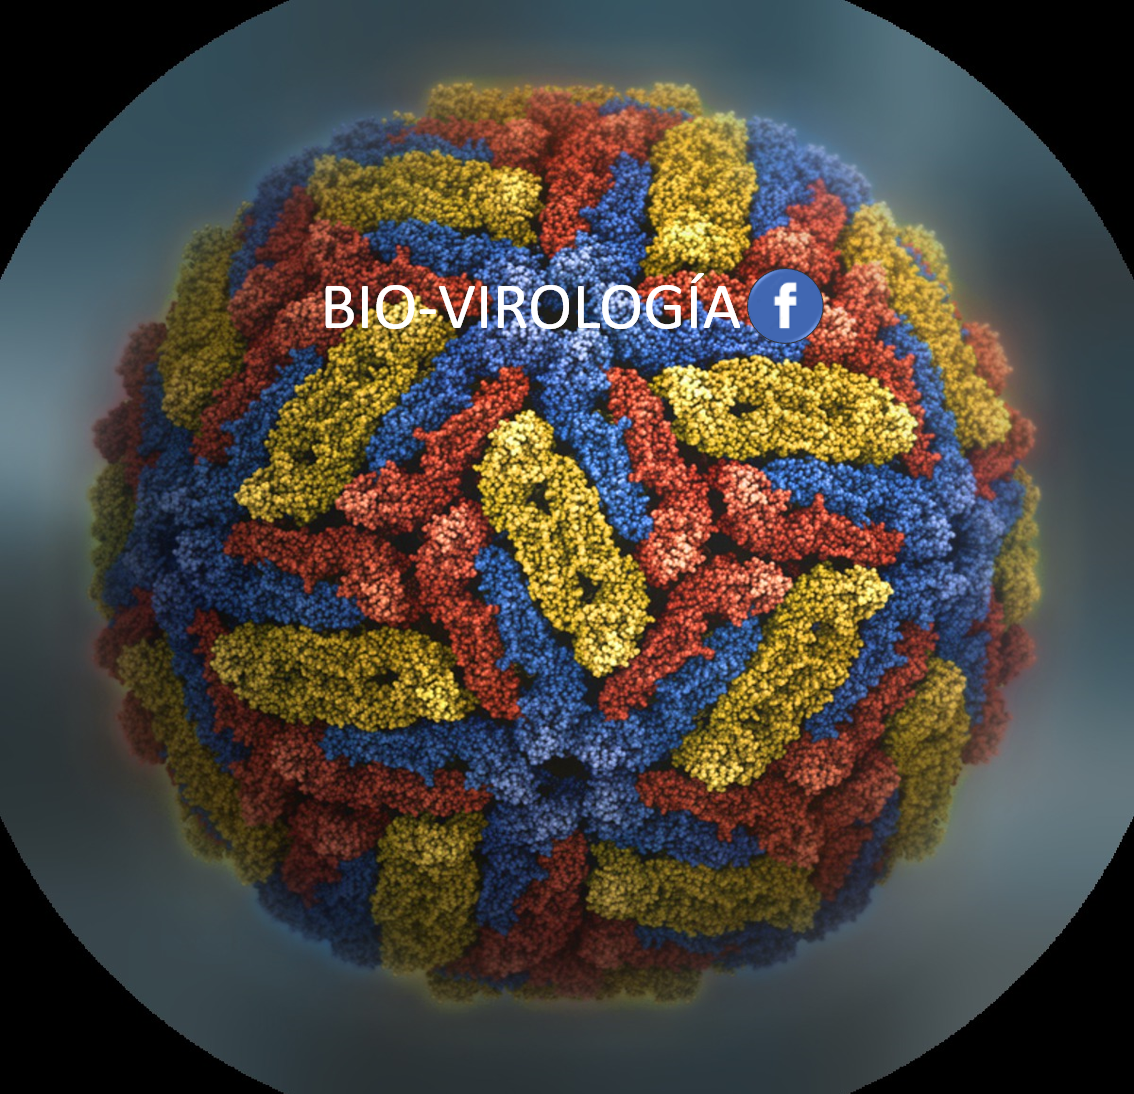
\includegraphics{figures/Portrait.gif}

El presente Bookdown es un el producto de la integración de tres medios de divulgación científica en formato de Blog en Facebook: \href{https://www.facebook.com/BioViral/}{Biovirología}, \href{https://www.facebook.com/Mimivirus-100736401569015}{Mimivirus} y \href{https://www.facebook.com/Medicina88}{Quantum Rabbit}. En el que re-lanzamos e inmortalizamos los contenidos desarrollados en las tres páginas bajo el formato nada tradicional de libro electrónico interactivo: Bookdown, un formato web con las características de los libros electrónicos clásicas -consultable en pdf, epub- y disponible para celular, tablet u ordenador de escritorio, junto con todas las posibilidades de edición y de contenido de un sitio web. Por lo que en este formato se puede escribir, editar y hasta interactuar con los lectores, además de insertar gráficas, videos, animaciones (como nuestra portada, que por cierto representa el \href{https://www.ebi.ac.uk/pdbe/entry/search/index/?searchParams=\%7B\%22q_scop_family\%22:\%5B\%7B\%22value\%22:\%22Virus\%20envelope\%20proteins\%22,\%22condition1\%22:\%22AND\%22,\%22condition2\%22:\%22Contains\%22\%7D\%5D,\%22resultState\%22:\%7B\%22tabIndex\%22:0,\%22paginationIndex\%22:1,\%22perPage\%22:\%2210\%22,\%22sortBy\%22:\%22Sort\%20by\%22\%7D\%7D}{virión del virus Dengue}', hecho animación en \href{https://ezgif.com/video-to-gif}{Ezgif}; códigos escritos en los lenguajes de programación R, bash, perl, python (entre otros), o emplear, incluso, comandos del lenguaje estructurado TeX (con el que se generan documentos LaTex). Funcionando por tanto como un notebook en el que se puede visualizar el output o la salida de los códigos en él escritos. Así, con esta transición el producto de integración de estos tres blogs de divulgación científica en español es el primer bookdown de divulgación científica en español, además del primero en virología biológica o biovirología.

\hypertarget{autores}{%
\subsection*{Autores}\label{autores}}
\addcontentsline{toc}{subsection}{Autores}

\begin{itemize}
\item
  \textbf{Aimer G. Díaz}: MSc. Bioinformático y Biólogo de la Universidad Nacional de Colombia. Fundador del blog de divulgación de virología biológica o no-médica ``Bio-Virología''. Co-fundador, escritor y editor del blog de divulgación científica \href{https://bioteorica.wixsite.com/bioteorica/blog}{Biología Teórica para T@dos} (En \href{https://www.facebook.com/BioTeoricaParaTodos/}{Facebook}), además de escribir para \href{http://www.biologiamolecularmexico.com/}{Biología Molecular México} (En \href{https://www.facebook.com/biologiamolecularmexico/}{Facebook}). Actualmente estudiante de doctorado y miembro investigador del Centro para el estudio de la evolución en acción BEACON. Los ejes temáticos en los que se concentra su investigación y divulgación científica son Virología, Bioinformática, Biología Evolutiva y Filosofía de la Biología, pese a la diversidad de áreas todas estas convergen alrededor de la Virología evolutiva computacional.
\item
  \textbf{Víctor Parra Avellaneda}: Estudia la licenciatura en Biología en el Centro Universitario de Ciencias Biológicas y Agropecuarias de la Universidad de Guadalajara. Fundador del blog de divulgación científica Mimivirus \href{https://www.facebook.com/Mimivirus-100736401569015}{(en Facebook)}, enfocado en virología. Los ejes temáticos abordados en su divulgación científica son la virología, ingeniería genética, microbiología y biología sintética. Por otra parte, también se desempeña en el ámbito literario, específicamente en la ciencia ficción. Es autor de la novela satírica El intrigante caso de Locostein, (Editorial Dreamers, 2019), ha publicado sus relatos en revistas literarias como Axxón, Marabunta, Penumbria, Sci:fdI (revista de la Universidad Complutense de Madrid), Almiar; en inglés en las revistas The Temz Review, Nymphs y Teleport Magazine; y en francés en Dumas de demain. Fue becario del PECDA Nayarit 2018-2019 en la categoría de cuento. Es fundador y co-editor de la revista literaria de ficción especulativa Primero Sueño.
\item
  \textbf{Juan Corao}: Biólogo con especialidad en biología celular de la Universidad de los Andes, Mérida, Venezuela. Como profesional siempre ha buscado un enfoque multidisciplinario e integrativo dirigido a la conservación de la biodiversidad y agro-biodiversidad, realizando múltiples trabajos de asesoramiento ambiental en manejo de fuentes y nacientes de agua en distintos ecosistemas y países, así como en el diseño de planes de manejo ambiental para múltiples fines. Ha trabajado como asesor para la empresa privada, ONU mujeres Ecuador, Instituto Nacional de Investigaciones Agrícolas INIA Venezuela. También maneja una empresa de generación de semillas de hongos comestibles y distintos bioinsumos para el sector agrícola. Actualmente es profesor de genética en el departamento de Biología, Facultad de Ciencias, Universidad de los Andes, Mérida Venezuela. Sus intereses académicos tienen que ver con la metagenómica aplicada a la conservación y al monitoreo del cambio climático y su impacto en la biodiversidad. Para el 2022 comienza un doctorado en ecología tropical en el Instituto de Ciencias Ambientales y Ecológicas ICAE, ULA.
\item
  \textbf{Roberto Nájera}: Autodidacta en Biología molecular, fisiología, farmacología, cinética enzimática y biología de sistema. Fundador del blog \href{https://www.facebook.com/Medicina88}{Quantum Rabbit} de divulgación científica y del canal homonimo de animaciones científicas de procesos fisiológicos y bioquímicos en \href{https://www.youtube.com/channel/UC21O3WpoUEXuu6ZmvkFHOCA}{YouTube}. Sus intereses radican en especial en la compresión del Envejecimiento, cáncer, Bio-ingeniería de proteínas y Modelación matemática del metabolismo celular.
\item
  \textbf{Natalia Alejandra Chaparro}: Magíster en Filosofía de la Universidad Nacional de Colombia con licenciatura en español y filología clásica. Bajo el cobijo del amor a la sabiduría, Natalia busca conocer y reflexionar la vida con todas sus particularidades.
\end{itemize}

\hypertarget{interacciuxf3n}{%
\subsection*{Interacción}\label{interacciuxf3n}}
\addcontentsline{toc}{subsection}{Interacción}

¿Deseas comentar, corregir, sugerir, opinar o preguntar algo sobre el \texttt{Bookdown}? Puedes hacerlo \href{https://github.com/AimerGDiaz/Bio-Virologia/discussions/10}{en esta sección}.

\hypertarget{licencia}{%
\subsection*{Licencia}\label{licencia}}
\addcontentsline{toc}{subsection}{Licencia}

Este obra está protegida bajo una licencia de \href{https://creativecommons.org/licenses/by-nc-nd/4.0/deed.es_ES}{Creative Commons Reconocimiento-NoComercial-SinObraDerivada 4.0 Internacional}

\href{https://creativecommons.org/licenses/by-nc/4.0/}{\includegraphics{https://img.shields.io/badge/License-CC\%20BY--NC\%204.0-lightgrey.svg}}

\hypertarget{contenido-del-blog-en-facebook-en-proceso-de-migraciuxf3n}{%
\subsection*{Contenido del blog en facebook en proceso de migración}\label{contenido-del-blog-en-facebook-en-proceso-de-migraciuxf3n}}
\addcontentsline{toc}{subsection}{Contenido del blog en facebook en proceso de migración}

\textbf{Lista de post publicados en} \href{https://www.facebook.com/permalink.php?story_fbid=174758050915684\&id=107088044349352}{Facebook}

\begin{enumerate}
\def\labelenumi{\arabic{enumi}.}
\item
  Virus que embellecen la primavera. \protect\hyperlink{vircolor}{Bookdown}, \href{https://www.facebook.com/BioViral/posts/166521528808498}{Facebook}
\item
  El viroma humano. \protect\hyperlink{viroma}{Bookdown}, \href{}{Facebook}
\end{enumerate}

2.1 El viroma del genoma humano. \protect\hyperlink{viroma_genoma}{Bookdown}, \href{https://www.facebook.com/permalink.php?story_fbid=108452037546286\&id=107088044349352}{Facebook}

2.2 ¿Somos híbridos entre virus y humanos? \protect\hyperlink{hybrids}{Bookdown}, \href{https://www.facebook.com/BioViral/posts/152069863586998}{Facebook}

\begin{enumerate}
\def\labelenumi{\arabic{enumi}.}
\setcounter{enumi}{2}
\tightlist
\item
  ¿Es posible visualizar viriones o virus? \protect\hyperlink{viralSigns}{Bookdown}
\end{enumerate}

3.1 Podemos ver los síntomas que causa su infección en los Tulipanes \protect\hyperlink{tulipomania}{Bookdown}, \href{https://www.facebook.com/permalink.php?story_fbid=116167563441400\&id=107088044349352}{Facebook}

\begin{enumerate}
\def\labelenumi{\arabic{enumi}.}
\setcounter{enumi}{3}
\item
  Metafísica y Virología: Los virus desde la ontología de Procesos \protect\hyperlink{metafisica}{Bookdown}, \href{https://www.facebook.com/permalink.php?story_fbid=137306747994148\&id=107088044349352}{Facebook}
\item
  ¿Qué son los virus? ¿Genes escapados, células reducidas o las primeras células que se dispersan con ``semillas''? \protect\hyperlink{WhatVirusAre}{Bookdown}, \href{https://www.facebook.com/permalink.php?story_fbid=145223737202449\&id=107088044349352}{Facebook}
\item
  La extinción del virus de la viruela y el optimismo cientificista. \protect\hyperlink{viruela}{Bookdown}, \href{https://www.facebook.com/permalink.php?story_fbid=148436860214470\&id=107088044349352}{Facebook}
\end{enumerate}

\begin{enumerate}
\def\labelenumi{\arabic{enumi}.}
\setcounter{enumi}{6}
\tightlist
\item
  El año del SARS-CoV-2 \protect\hyperlink{sarscov2}{Bookdown}
\end{enumerate}

\begin{itemize}
\item
  ¿Siempre tienden los virus emergentes a atenuarse al adaptarse al nuevo huésped?. \href{}{Bookdown}, \href{https://www.facebook.com/permalink.php?story_fbid=164436058614550\&id=107088044349352}{Facebook}
\item
  ¿Por qué la letalidad del SARS-CoV-2 es diferente en la segunda ola de la pandemia?. \href{}{Bookdown}, \href{https://www.facebook.com/permalink.php?story_fbid=167096031681886\&id=107088044349352}{Facebook}
\item
  Rastreando la evolución de virus pandémicos en tiempo real. \href{}{Bookdown}, \href{https://www.facebook.com/permalink.php?story_fbid=169322844792538\&id=107088044349352}{Facebook}
\item
  SARS-COV-2 no saltó de una sopa. \href{}{Bookdown}, \href{https://www.facebook.com/permalink.php?story_fbid=172899017768254\&id=107088044349352}{Facebook}
\item
  40 a 70 años de evolución de SARS-CoV-2 en poblaciones de murciélagos de la provincia de Yunnan, China. \href{}{Bookdown}, \href{https://www.facebook.com/permalink.php?story_fbid=173344151057074\&id=107088044349352}{Facebook}
\item
  La cuarentena como esfuerzo colectivo e internacional funciona para contener la propagación de SARS-CoV-2. \href{}{Bookdown}, \href{https://www.facebook.com/BioViral/videos/810087529531891}{Facebook}
\item
  Más allá del rol anti-inmune de los polímeros de glicano en la proteína Spike del SARS-CoV-2 \href{}{Bookdown}, \href{https://www.facebook.com/BioViral/videos/952346028621514/}{Facebook}
\item
  Sindemia, Co-infecciones virales e Interferencia viral. \href{}{Bookdown}, \href{https://www.facebook.com/permalink.php?story_fbid=185807143144108\&id=107088044349352}{Facebook}
\item
  Hipótesis de Inmunidad basada en Diversidad Poblacional de los grupos ABO (IDP-ABO) \href{}{Bookdown}, \href{https://www.facebook.com/permalink.php?story_fbid=188174372907385\&id=107088044349352}{Facebook}
\item
  El punto de inflexión y el final de una epidemia en expansión no se puede pronosticar con precisión. \href{}{Bookdown}, \href{https://www.facebook.com/permalink.php?story_fbid=191562869235202\&id=107088044349352}{Facebook}
\item
  Mecanismo de evasión del reconocimiento del sistema inmune innato mediado por el robo de los antígenos ABO por parte del virus envuelto SARS-CoV-2 \href{}{Bookdown}, \href{https://www.facebook.com/BioViral/videos/4039190299441114/}{Facebook}
\item
  Definición y limites de Mutación, Polimorfismo, Infectividad, Virulencia, Patogenicidad e Inmunogenicidad. \href{}{Bookdown}, \href{https://www.facebook.com/permalink.php?story_fbid=191978355860320\&id=107088044349352}{Facebook}
\item
  Introducción a las vacunas adenovirales contra la COVID-19:

  \begin{itemize}
  \item
    ¿Por qué son tan utilizados los Adenovirus en el desarrollo de vacunas? Por Mimivirus \href{}{Bookdown}, \href{https://www.facebook.com/permalink.php?story_fbid=194256785632477\&id=107088044349352}{Facebook}
  \item
    ¿Por qué la vacuna rusa Sputnik V entró a fase III primero que todas las demás vacunas?. \href{}{Bookdown}, \href{https://www.facebook.com/permalink.php?story_fbid=194473115610844\&id=107088044349352}{Facebook}
  \end{itemize}
\item
  Introducción a las vacunas Experimentales basadas en mRNA. \href{}{Bookdown}, \href{https://www.facebook.com/permalink.php?story_fbid=195407762184046\&id=107088044349352}{Facebook}
\item
  El Nacionalismo de las vacunas \href{}{Bookdown}, \href{https://www.facebook.com/permalink.php?story_fbid=195747918816697\&id=107088044349352}{Facebook}
\item
  ¿Podemos confiar en una vacuna desarrollada en menos de 1 año? \href{}{Bookdown}, \href{https://www.facebook.com/permalink.php?story_fbid=210814357310053\&id=107088044349352}{Facebook}
\item
  La Sindemia de COVID-19 se enfrentará empleando vacunas de nueva generación. \href{}{Bookdown}, \href{https://www.facebook.com/permalink.php?story_fbid=211176330607189\&id=107088044349352}{Facebook}
\item
  ¿Cómo se ha reducido el tiempo para producir la vacuna contra la COVID-19 de 5 o 10 años a menos de 1 año? \href{}{Bookdown}, \href{https://www.facebook.com/BioViral/videos/437319657293716/}{Facebook}
\item
  El origen del virus SARS-CoV-2 es natural, pero el ser humano propició las condiciones ambientales para que este, y otros virus, emerjan. \href{}{Bookdown}, \href{https://www.facebook.com/permalink.php?story_fbid=215833596808129\&id=107088044349352}{Facebook}
\item
  Reporte del significado de la sustitución E484K de la proteína Spike. \href{}{Bookdown}, \href{https://www.facebook.com/permalink.php?story_fbid=238010707923751\&id=107088044349352}{Facebook}

  \begin{itemize}
  \item
    ¿Cuándo una mutación cobra interés para los científicos?, ¿Cuándo cobra interés para el público en general?. \href{}{Bookdown}, \href{https://www.facebook.com/permalink.php?story_fbid=238575207867301\&id=107088044349352}{Facebook}
  \item
    Clasificación, semejanzas y diferencias entre los dos tipos de vectores de las principales vacunas contra COVID-19. \href{}{Bookdown}, \href{https://www.facebook.com/permalink.php?story_fbid=241254277599394\&id=107088044349352}{Facebook}
  \end{itemize}
\item
  Primeros resultados de la vacunación masiva con BNT162b2 de Pfizer/Biontech en Israel. \href{}{Bookdown}, \href{https://www.facebook.com/permalink.php?story_fbid=244379250620230\&id=107088044349352}{Facebook}
\item
  La vacuna Gam-COVID-Vac tiene una eficacia del 91,6\% (N= 19866 voluntarios) y de 91,8\% en mayores de 60 años (N = 2144), datos preliminares. \href{}{Bookdown}, \href{https://www.facebook.com/permalink.php?story_fbid=249885460069609\&id=107088044349352}{Facebook}
\item
  La eficacia de las vacunas adenovirales varia en función de la incidencia y el tipo de adenovirus circulantes de cada región. \href{}{Bookdown}, \href{https://www.facebook.com/permalink.php?story_fbid=250473223344166\&id=107088044349352}{Facebook}
\item
  Los hábitos de higiene y distanciamiento social adquiridos por la Sindemia de COVID-19 tienen el potencial de afectar el microbioma humano. \href{}{Bookdown}, \href{https://www.facebook.com/permalink.php?story_fbid=257922015932620\&id=107088044349352}{Facebook}
\item
  Primeros reportes sobre la respuesta inmune celular o mediada por células T frente a las nuevas variantes de SARS-CoV-2.\href{}{Bookdown}, \href{https://www.facebook.com/permalink.php?story_fbid=258465985878223\&id=107088044349352}{Facebook}
\item
  ¿Cómo se asignan los nombres para los nuevos linajes de SARS-CoV-2?. \href{}{Bookdown}, \href{https://www.facebook.com/BioViral/videos/841733049886877/}{Facebook}
\item
  Eficacia y características de 9 vacunas contra COVID-19. \href{}{Bookdown}, \href{https://www.facebook.com/permalink.php?story_fbid=267375121653976\&id=107088044349352}{Facebook}
\item
  La eficacia y la efectividad de una vacuna NO es lo mismo. \href{}{Bookdown}, \href{https://www.facebook.com/permalink.php?story_fbid=285011853223636\&id=107088044349352}{Facebook}
\item
  ``Test rápidos de antígenos para detectar a los más contagiosos'' \href{}{Bookdown}, \href{https://www.facebook.com/permalink.php?story_fbid=285058139885674\&id=107088044349352}{Facebook}
\item
  ¿Requieren regulación basada en evidencia los esfuerzos de confinamiento?. \href{}{Bookdown}, \href{https://www.facebook.com/BioViral/videos/442313850196495/}{Facebook}
\item
  ¿Cómo se evitó la pandemia de SRAS en el 2002, enfermedad causada por el coronavirus SARS-CoV?. \href{}{Bookdown}, \href{https://www.facebook.com/BioViral/posts/155212829939368}{Facebook}
\item
  ¿Qué falló en el control de la pandemia de COVID-19 causada por SARS-CoV-2? \href{}{Bookdown}, \href{https://www.facebook.com/BioViral/posts/171521324975185}{Facebook}
\item
  El virus SARS-CoV-2 NO causa el fenómeno de ``Amplificación de la infección dependiente de anticuerpos''. \href{}{Bookdown}, \href{https://www.facebook.com/BioViral/posts/175339871259997}{Facebook}
\item
  Las manifestaciones masivas no aumentan dramáticamente la tasa de contagios de COVID-19. \href{}{Bookdown}, \href{https://www.facebook.com/BioViral/posts/175382534589064}{Facebook}
\item
  La vacuna de mRNA ``CVnCoV'' termo-resistente y de alto rendimiento de CureVac. \href{}{Bookdown}, \href{https://www.facebook.com/BioViral/posts/185658043561513}{Facebook}
\item
  ¿Por qué las vacunas intramusculares no previenen el contagio de COVID-19?. \href{}{Bookdown}, \href{https://www.facebook.com/BioViral/posts/201146022012715}{Facebook}
\item
  La efectividad de la vacuna de Sinovac en el mundo real es mucho mejor que la eficacia reportada en los ensayos clínicos: Del 51\% al 67\%. \href{}{Bookdown}, \href{https://www.facebook.com/BioViral/posts/202619181865399}{Facebook}
\item
  ``¡Refuerzo de BNT162b2 (Pfizer/BioNTech), aún no gracias!''. \href{}{Bookdown}, \href{https://www.facebook.com/BioViral/posts/206887918105192}{Facebook}
\end{itemize}

\begin{enumerate}
\def\labelenumi{\arabic{enumi}.}
\setcounter{enumi}{7}
\tightlist
\item
  Geometría de viriones los sólidos platónicos de la naturaleza. \href{}{Bookdown}
\end{enumerate}

8.1 Adenovirus y sus viriones de geometría poliédrica T=25. \href{}{Bookdown}, \href{https://www.facebook.com/permalink.php?story_fbid=162961568761999\&id=107088044349352}{Facebook}

\begin{enumerate}
\def\labelenumi{\arabic{enumi}.}
\setcounter{enumi}{8}
\tightlist
\item
  Monitoreo de la evolución de SARS-CoV-2 en tiempo real \href{}{Bookdown}
\end{enumerate}

9.1 Evolución en tiempo real por selección natural en SARS-CoV-2. \href{}{Bookdown}, \href{https://www.facebook.com/permalink.php?story_fbid=176697107388445\&id=107088044349352}{Facebook}

9.2 Indicios de convergencia evolutiva por selección natural en tres linajes de SARS-CoV-2 portadores de la variante N501Y. \href{}{Bookdown}, \href{https://www.facebook.com/permalink.php?story_fbid=249352400122915\&id=107088044349352}{Facebook}

9.3 Homenaje Virológico a Charles Robert Darwin por su cumpleaños número 212 (12 de Febrero de 1809). \href{}{Bookdown}, \href{https://www.facebook.com/permalink.php?story_fbid=257534675971354\&id=107088044349352}{Facebook}

9.4 Evolución de Cuasiespecies. \href{}{Bookdown}, \href{https://www.facebook.com/BioViral/posts/180308757429775}{Facebook}

9.5 Del árbol evolutivo de SARS-CoV-2 siguen brotando nuevas ramas. Lo que no significa necesariamente que las vacunas ya no funcionen. \href{}{Bookdown}, \href{https://www.facebook.com/BioViral/posts/200426228751361}{Facebook}

9.6 Tasa de propagación, primeros reportes del efecto sobre las vacunas de la variante Delta y la falsa concepción de progreso en la evolución del SARS-CoV-2. \href{}{Bookdown}, \href{https://www.facebook.com/BioViral/posts/213300734130577}{Facebook}

\begin{enumerate}
\def\labelenumi{\arabic{enumi}.}
\setcounter{enumi}{9}
\item
  Mimivirus y el descubrimiento de virus gigantes (por Víctor Avellaneda). \href{}{Bookdown}, \href{https://www.facebook.com/permalink.php?story_fbid=148814966843326\&id=107088044349352}{Facebook}
\item
  El árbol de la vida debe incluir a los virus tanto en su raíz y sus ramas. \href{}{Bookdown}
\end{enumerate}

11.1 LUCA como comunidad heterogénea de linajes. \href{}{Bookdown}, \href{https://www.facebook.com/permalink.php?story_fbid=180759156982240\&id=107088044349352}{Facebook}

11.2 Nada escapa de los virus, ni siquiera ellos mismos. \href{}{Bookdown}, \href{https://www.facebook.com/permalink.php?story_fbid=216494243408731\&id=107088044349352}{Facebook}

11.3 La hipótesis del origen viral del ADN. \href{}{Bookdown}, \href{https://www.facebook.com/BioViral/posts/218632920264025}{Facebook}

\begin{enumerate}
\def\labelenumi{\arabic{enumi}.}
\setcounter{enumi}{11}
\tightlist
\item
  Mutualismo entre organismos celulares y virales \href{}{Bookdown}
\end{enumerate}

12.1 Los virus gigantes Coanovirus podrían otorgar a sus huéspedes heterótrofos Coanoflagelados capacidades foto-heterotróficas.\href{}{Bookdown}, \href{https://www.facebook.com/permalink.php?story_fbid=184190396639116\&id=107088044349352}{Facebook}

\begin{enumerate}
\def\labelenumi{\arabic{enumi}.}
\setcounter{enumi}{12}
\item
  El intercambio de especies entre el Viejo y el Nuevo Mundo. \href{}{Bookdown}, \href{https://www.facebook.com/permalink.php?story_fbid=184862273238595\&id=107088044349352}{Facebook}
\item
  Los Virus como entidades hipervariables a nivel de la biología molecular.
\end{enumerate}

14.1 La Belleza, excepcionalidad y diversidad de los genomas virales. \href{}{Bookdown}, \href{https://www.facebook.com/permalink.php?story_fbid=193816995676456\&id=107088044349352}{Facebook}

14.2 ¿Qué son los genes superpuestos?. \href{}{Bookdown}, \href{https://www.facebook.com/permalink.php?story_fbid=215736123484543\&id=107088044349352}{Facebook}

\begin{enumerate}
\def\labelenumi{\arabic{enumi}.}
\setcounter{enumi}{14}
\tightlist
\item
  El Dilema Inmunológico del Origen de la Placenta en Mamíferos. \href{}{Bookdown}
\end{enumerate}

15.1 El origen viral de la placenta: la historia sobre cómo en el trofoblasto proteínas derivadas de retrovirus permiten la invasión del endometrio materno. \href{}{Bookdown}, \href{https://fb.watch/3nTBh_kCbc/}{Facebook}

15.2 La proteína de origen viral, Sincitina-1, confiere capacidad inmunosupresora y permite la invasión del endometrio materno. \href{}{Bookdown}, \href{https://fb.watch/47zn4aTTy9/}{Facebook}

\begin{enumerate}
\def\labelenumi{\arabic{enumi}.}
\setcounter{enumi}{15}
\tightlist
\item
  Ecología viral. \href{}{Bookdown}
\end{enumerate}

16.1. Los virus gobiernan el clima oceánico mundial. \href{}{Bookdown}, \href{https://www.facebook.com/BioViral/videos/2866496176923128/}{Facebook}

\begin{enumerate}
\def\labelenumi{\arabic{enumi}.}
\setcounter{enumi}{16}
\tightlist
\item
  La extraña y estrecha relación entre los virus y los ARNs de transferencia. \href{}{Bookdown}
\end{enumerate}

17.1 La bacteria sintética Syn61 (\emph{E. coli}) es el primer organismo inmune a cualquier infección viral. \href{}{Bookdown}, \href{https://www.facebook.com/BioViral/posts/177374761056508}{Facebook}

\begin{enumerate}
\def\labelenumi{\arabic{enumi}.}
\setcounter{enumi}{17}
\tightlist
\item
  Sistemas de inmunidad antiviral de origen viral \href{}{Bookdown}
\end{enumerate}

18.1. Cas-9 filmado en acción a escala y tiempo real mediante microscopia de fuerza atómica de alta velocidad. \href{}{Bookdown}, \href{https://www.facebook.com/BioViral/posts/191468236313827}{Facebook}

\begin{enumerate}
\def\labelenumi{\arabic{enumi}.}
\setcounter{enumi}{18}
\tightlist
\item
  Domesticación viral y el kit de herramientas del biólogo molecular \href{}{Bookdown}
\end{enumerate}

19.1 ¿Qué papel juega el virus de la hepatitis B en la vacuna contra la malaria ``RTS,S''? {[}Bookdown{]}{[}\#malariaVaccine{]}\href{}{Facebook}

\hypertarget{prefacio}{%
\section*{Prefacio}\label{prefacio}}
\addcontentsline{toc}{section}{Prefacio}

El presente bookdown se une a la serie de obras contemporáneas cuya marca distintiva a los formatos tradicionales radica en el hecho de la obra está intencionalmente inacabada, en constante desarrollo, revisión y edición (aún en esta etapa inicial de selección y migración del contenido de las paginas en Facebook).

Los bookdown son como tal proyectos web que se han descrito como ``never-ending work-in-progress'' -trabajo interminable en progreso- o ``ever-growing-work'' -trabajo en constante crecimiento-, entre los proyectos destacados que se han realizado bajo este formato se destacan \href{https://compgenomr.github.io/book/}{Computational Genomics with R}, \href{https://epirhandbook.com/en/index.html}{The Epidemiologist R Handbook} entre otros que puede ser consultados en el sitio oficial de los \href{https://bookdown.org/home/archive/}{bookdowns}.

Formatos adicionales por ejemplo son los revolucionarios libros de biología molecular interactivos y animados como \href{https://www.smart-biology.com/}{Smart-Biology} o herramientas bibliográficas como la modesta pero sorprendente red de aprobación - complementación o reprobación - refutación entre tesis de prominentes autores de la historia de la filosofía de la biología
``\href{https://www.denizcemonduygu.com/philo/}{History of philosophy: summarized \& visualized}''.

En la presente obra integraremos no solo texto e imágenes divulgativas en relación a la biología de los virus, sino que además emplearemos modelos animados basados en evidencia, bajo el característico estilo de \href{https://www.facebook.com/Medicina88}{Quatum Rabiit}, pero por ahora, a manera introductoria de las maravillas del formato Bookdown, los invito a ver el siguiente vídeo, que a su vez, permite introducir a uno de los autores del presente documento:

\href{http://www.youtube.com/watch?v=EmEhFhQpqTQ}{\includegraphics{http://img.youtube.com/vi/EmEhFhQpqTQ/0.jpg}}

Entrevista para Ciencia café, pa' Sumercé: ``En la coloración de las plantas: 1 + 1 no es 2''.

\hypertarget{descripciuxf3n-de-la-obra}{%
\subsection*{Descripción de la obra}\label{descripciuxf3n-de-la-obra}}
\addcontentsline{toc}{subsection}{Descripción de la obra}

La presente obra nace como parte del proyecto de Biovirología, que inició en un nada remoto \href{https://www.facebook.com/permalink.php?story_fbid=107125457678944\&id=107088044349352}{19 de mayo del 2020} en el contexto de la Sindemia de COVID-19, bajo la fuerte influencia de la labor de divulgación del blog ``Mimivirus''. De allí que el proyecto partió como un medio adicional para combatir la desinformación que caracterizaron la infodemia relacionada a la pandemia, pero ha ido evolucionado hacia la reinvidicación de ecológica y evolutiva de los virus como entidades escenciales en la trama de la vida.

El primero post de aquella fecha es reproducido a continuación:

Inauguro este espacio de divulgación científica en español sobre artículos de investigación en virología desde una perspectiva netamente biológica. En este espacio los virus no solo serán agentes etiológicos o factores causales de enfermedades en humanos; en vez de esto, se discutirán como los virus en su función ecosistémica como nanobiota son componentes esenciales de los organismos en los que habitan -viroma-, como también de los ecosistemas en los que estos se transmiten -virósfera-.

Sobra decirlo, a la pregunta si los virus ¿ viven o no ?. La respuesta es un contundente Si, en palabras del virólogo Francés Patrick Forterre:

\begin{quote}
``(Los) virus no deben confundirse con sus viriones, sino que se pueden ver como entidades vivientes complejas que transforman la célula infectada en un organismo nuevo, el virus, que produce viriones.''
\end{quote}

\begin{quote}
``Viruses are no more confused with their virions, but can be viewed as complex living entities that transform the infected cell into a novel organism---the virus---producing virions'' \citet{forterre2010defining}
\end{quote}

Por la anterior cita, las historias que se contarán serán sobre las fábricas virales (viriones replicantes o viriones germinados en el recurso celular), como producto del curso exitoso de la infección, que es a su vez el establecimiento de las virocélulas (virocells). Y aunque nuestra portada refleja el énfasis clásico sobre las semillas proteicas (viriones), el objetivo de tal imagen es representar la concepción usual de lo que se cree que es un virus, que en especial refleja a propósito los colores de la bandera del país de origen de varios autores:

\begin{figure}
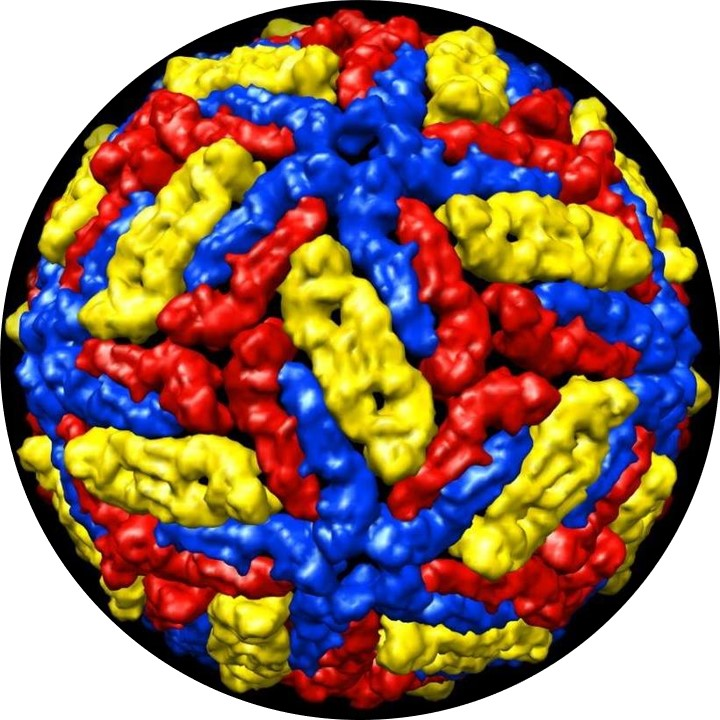
\includegraphics[width=0.5\linewidth]{Logo} \caption{Partícula viral o virión del virus del Nilo Occidental con los colores del la bandera de Colombia en homenaje al 3 encuentro panamericano de Dengue celebrado en Cartagena Colombia. Tomado de @mukhopadhyay2003structure}\label{fig:index2}
\end{figure}

\hypertarget{WhatVirusAre}{%
\section{¿Qué son los virus?}\label{WhatVirusAre}}

\textbf{¿Genes escapados, células reducidas o las primeras células que se dispersan con ``semillas''? }

El debate en torno a si los \textbf{virus son o no entidades vivientes (1)} usualmente trae a discusión cuatro preguntas adicionales y relacionadas: \textbf{¿Qué es la vida? (2)}, \textbf{¿Qué son los virus? (3)}, \textbf{¿Forman los virus su propio árbol de la vida? (4)} y \textbf{¿Son los virus una clase natural}, semejante por ejemplo a cuando hablamos de primates quienes han evolucionado a partir de un único ancestro, \textbf{o es una clase artificial? (5)}. Y aunque pareciese que estas preguntas debiesen responderse en el orden descrito, los resultados de investigación nacen en cualquier dirección, lo que complica aún más presentar una respuesta única a la pregunta inicial.

Existen 3 escenarios diferentes alternativos que proveen respuestas diferentes a las 5 preguntas previamente planteadas (Figura 1). Empezado por el modelo más popular pero más debatido en los últimos años: \textbf{los virus son un conjunto de genes parásitos fugados de entidades celulares (3)}, es decir con capacidad de replicarse a sí mismos a expensas de la replicación de un organismo huésped. En esta interpretación, \textbf{los virus no son entidades vivas (1)}, pues carecen del \textbf{metabolismo celular autónomo y la maquinaria de traducción que produce las proteínas que llevan su propia replicación (2)}, y a diferencia de los parásitos celulares obligados, como algunas bacterias que también dependen de otros organismos para su reproducción y metabolismo, los virus, al descender de genes escapados no han tenido en toda su historia evolutiva la información necesaria para estas funciones, \textbf{de hecho por su origen celular carecen de un ancestro único y no representan un único linaje evolutivo (4)}, su evolución es completamente dependiente de la evolución de las células que parásita. Es por esto que los virus \textbf{como conjunto de replicadores no es una clase natural} y se agrupan artificialmente o por motivos explicativos por la similitud en su estrategia de propagación mediante viriones (5).

\begin{figure}
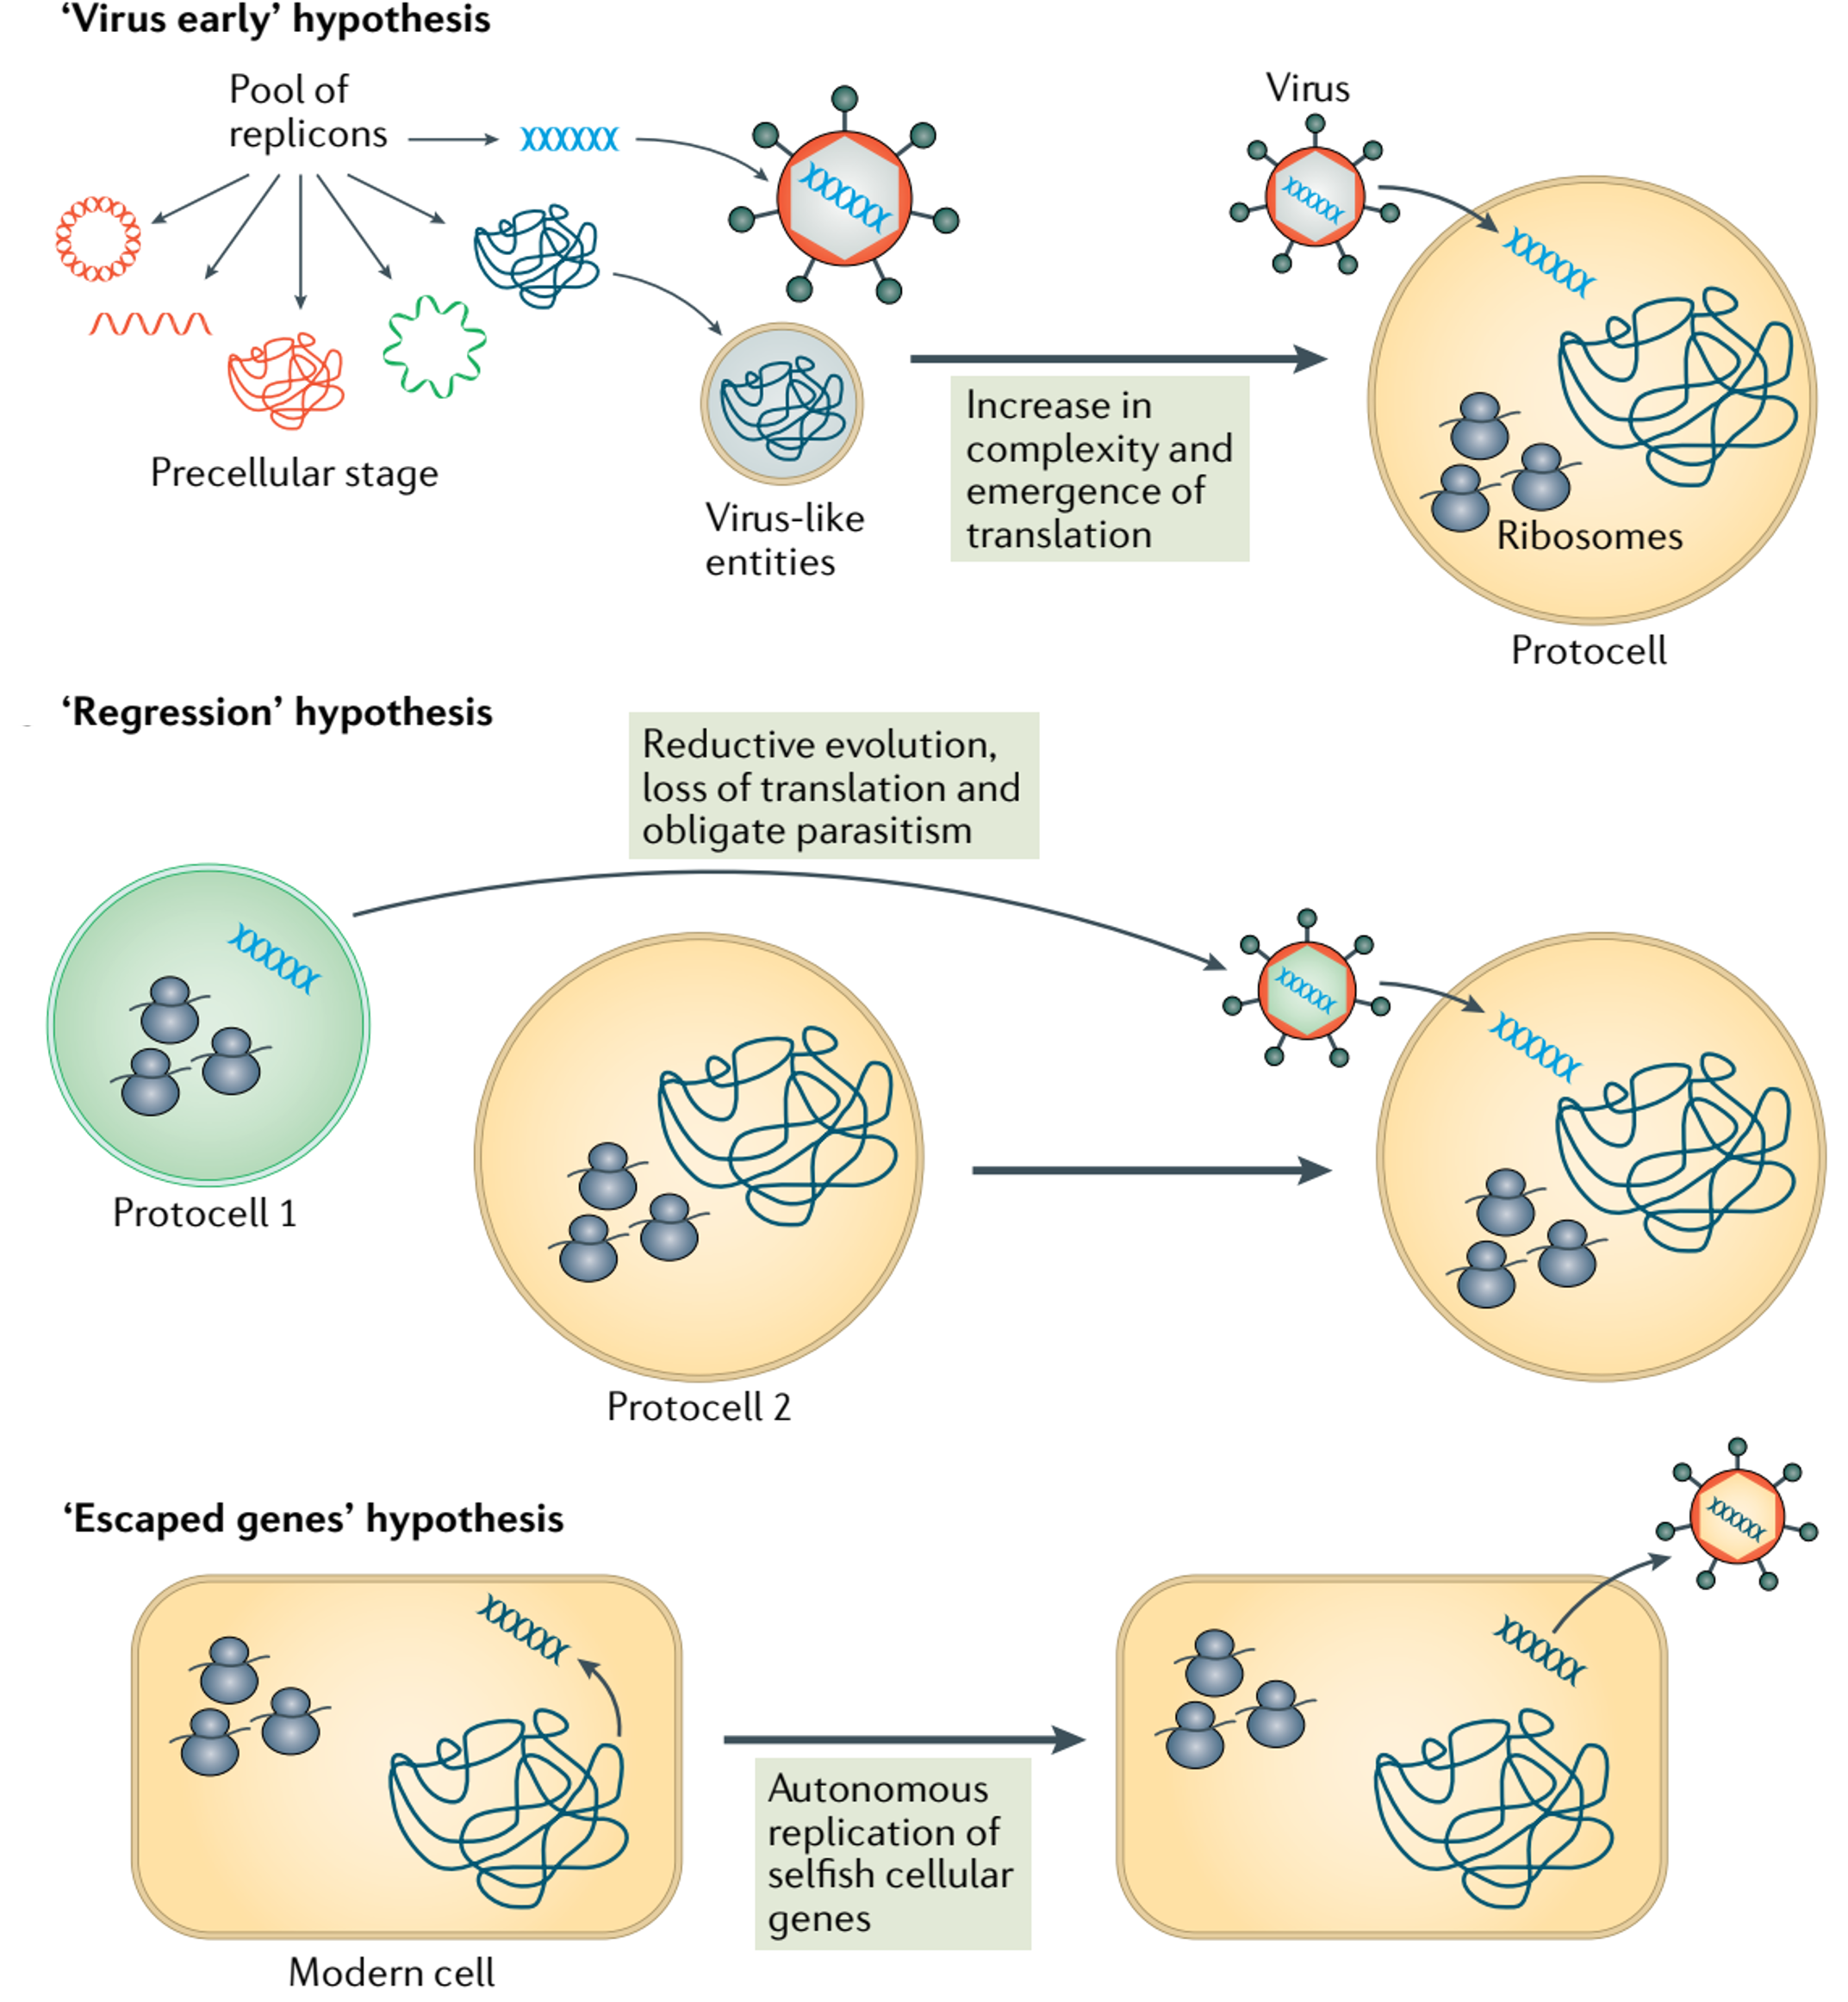
\includegraphics[width=0.8\linewidth]{figures/threeHypo} \caption{Los tres principales escenarios alternativos a las cinco preguntas planteadas al iniciar la discusión del presente segmento. Imagen tomada y modifica de @krupovic2019origin}\label{fig:threehypo}
\end{figure}

Tres descubrimientos recientes han puesto en duda las 5 respuestas del modelo centrado en el virus como genes escapados en vehículos llamados viriones: \textbf{(1) El descubrimiento de virus gigantes}, incluso tan grandes como la bacteria \emph{E. coli} (\textasciitilde2um), el caso del enigmático \emph{Pithovirus} (\textasciitilde1.5um) (Figura 2). El cual cuenta con una complejidad genética única e incluso con un tamaño mayor al de bacterias parásitas obligadas (\emph{Mycoplasma pneumoniae} 0.8Mb vs \emph{Pandoravirus} 2.5Mb). (II) La existencia de virus que parasitan otros virus, el caso de los viriofagos, quienes no solo dependen de otros virus para replicarse (como los virus satélite), sino que van más allá y parasitan la fábrica viral o el centro de replicación del virus del cual dependen.

\begin{figure}
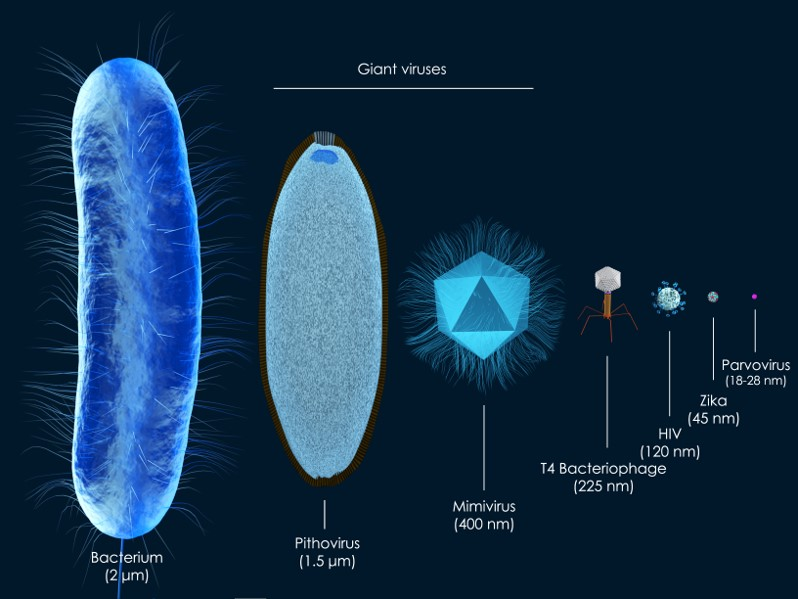
\includegraphics[width=0.8\linewidth]{figures/sizes} \caption{ Comparación del tamaño de la estrucutra dispersiva de diversos virus frente a la bacteria *E. coli*, creditos de la imagen a Meletios Verras stock illustration ID: 720441124}\label{fig:sizes}
\end{figure}

\begin{enumerate}
\def\labelenumi{(\Roman{enumi})}
\setcounter{enumi}{2}
\tightlist
\item
  La mayor dificultad al modelo de los virus como genes escapados en viriones es la \textbf{presencia de genes exclusivos a los virus}, como los genes que codifican las proteínas que forman las cápsides de los viriones o los responsables de la replicación del genoma viral, no obstante un descubrimiento fascinante en esta área ha demostrado que, aunque en su secuencia de ADN en virus de los 3 diferentes dominios (clásicos) de la vida (Bacteria, Arqueas y Eucariotas), NO hay evidencia de un único origen (o un ancestro viral común), esta tarea si es posible desde el punto de vista estructural de las proteínas de la cápside, como lo evidencia el plegamiento de los monómeros de la cápside de: Chlorella virus que infecta eucariotas, El bacteriófago PrD1 y el virus de arqueas termófilas STIV (Figura 3). El genoma de todos los anteriores virus es a base de ADN y de cadena doble, no obstante el dominio estructural llamado ``jelly-roll fold'' (o pliegue de gelatina) se encuentra en virus de cadena sencilla de ARN y ADN también, sugiriendo una historia evolutiva común (5) e independiente de la vida celular (4).
\end{enumerate}

\begin{figure}
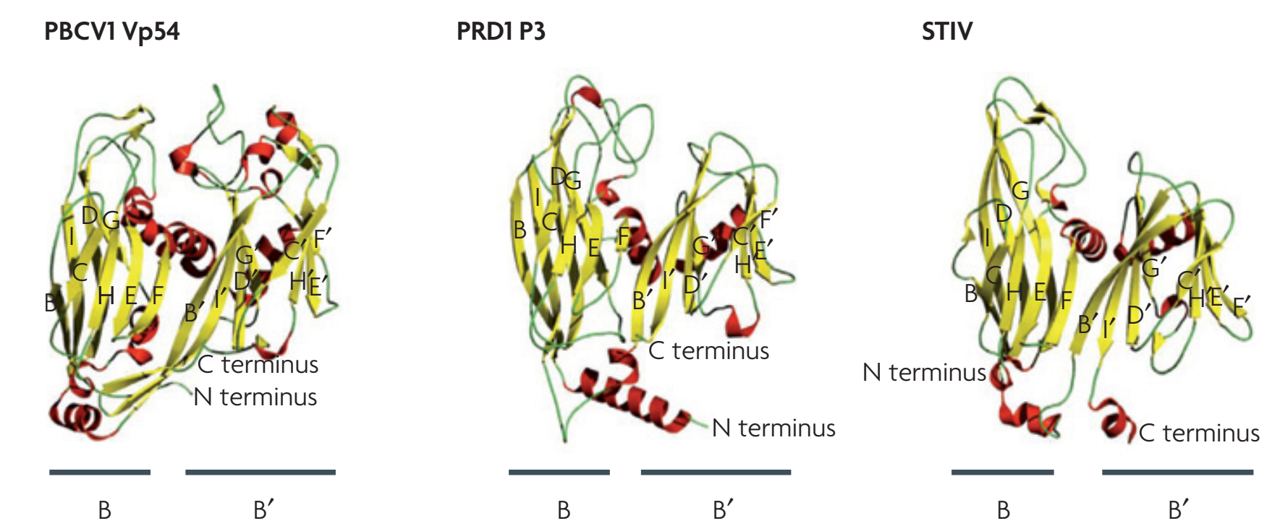
\includegraphics[width=0.8\linewidth]{figures/jelly-roll} \caption{Desde el punto de vista estructural de las proteínas de la cápside los virus parecen compartir un ancestro común, como lo evidencia el plegamiento de los monómeros de la cápside de: Chlorella virus que infecta eucariotas, El bacteriófago PrD1 y el virus de arqueas termófilas STIV, tomado de @raoult2008redefining}\label{fig:jellyroll}
\end{figure}

El modelo de reducción evolutiva sugiere que los virus representan un linaje evolutivo propio con características moleculares exclusivas y cuya historia evolutiva en el tiempo no se ha registrado en el ADN, pero si se evidencia en los plegamientos 3D de las proteínas que componen la cápside, los virus representarían una forma de vida propia derivada de un ancestro celular común, y por ende serían \textbf{manifestaciones vivas (1)} en forma de \textbf{parásitos obligados (3)} que precisamente roban la maquinaria de traducción de células mientras las parasitan. Este modelo se diferencia del escenario virus primero, en tanto que abarca solo aquellos virus a los que es posible rastrear una ancestría común, en cierto sentido el modelo de reducción evolutiva requiere el modelo de genes escapados para explicar ciertas familias virales atípicas o que carecen los plegamientos proteicos tipo ``jelly-roll fold''.En cambio, el modelo de virus primero no requiere qué estos hayan tenido alguna vez en la historia capacidad auto-replicativa autónoma ni la maquinaria de traducción para ser considerados vivos, sin embargo, la carencia de estas propiedades en el escenario del mundo de ARN no parece ser una anomalía. En esta narrativa lo que identifica a los virus como organismos vivos con un linaje único es la capacidad compartida de compactar y dispersar a manera de ``semillas'', \textbf{los viriones o partículas virales (VP)}, que almacenan el material genético necesario para tomar el control de células que codifican ribosomas, que a su vez portan un porcentaje de material genético adicional del cual los virus son capaces de controlar. De esta manera sí una célula con ribosomas es transformada germinaría la naturaleza celular de los virus, las \textbf{ribo-virocélulas}. En esta perspectiva el genoma de un virus está distribuido tanto en la semilla como en la célula huésped.

A manera de analogía Jean-Michel Claverie y Chantal Abergel proponen un cambio de perspectiva del ciclo de vida de los virus comparando su ciclo de vida con el de un mamífero capaz de leer y comprender estas letras, el humano, al igual que los virus, el ser humano emplea una estrategia dispersiva para heredar su genoma, los gametos (espermatozoides y óvulos), que son incapaces de sobrevivir autónomamente y que no portan la totalidad del genoma humano, sin embargo una vez dada la fecundación e implantación en un organismo huésped, inicia el programa de desarrollo de un organismo humano. Los gametos, en tanto son análogos a los viriones, son tan solo vehículos de un genoma parcial y compactado, más no son el organismo humano (Figura 4).

\begin{figure}
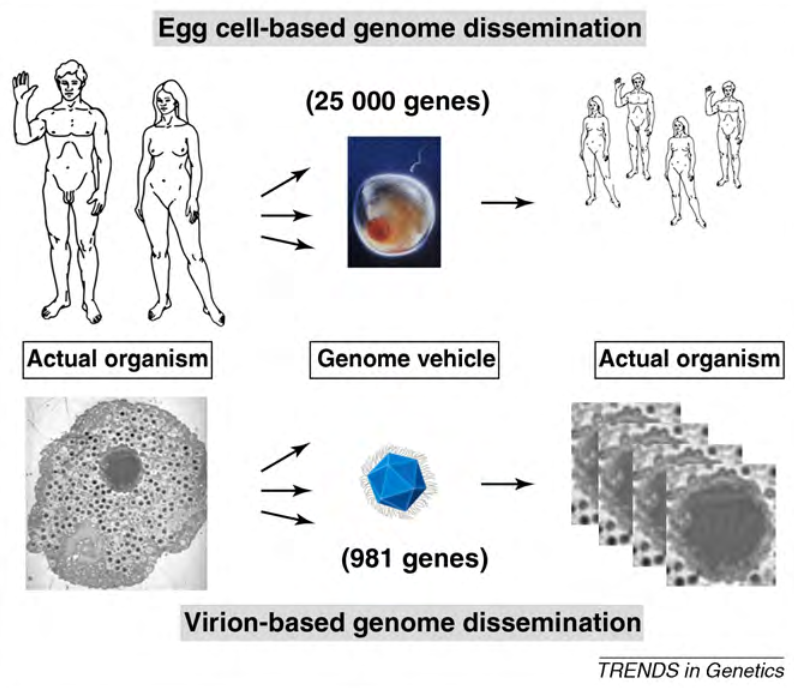
\includegraphics[width=0.8\linewidth]{figures/analogy} \caption{A manera de analogía @claverie2010mimivirus proponen un cambio de perspectiva del ciclo de vida de los virus, en el que al igual que en los humanos, existen etapas dispersivas en su ciclo de vida las cuales no son el enfoque a la hora de estudiar la fisología humana.}\label{fig:analogy}
\end{figure}

Compartenos tus respuestas en torno a estas preguntas \href{https://www.facebook.com/permalink.php?story_fbid=145223737202449\&id=107088044349352}{aquí}. ¿Consideran que es hora de replantearse el escenario de genes fugados?, ¿Cómo explicar con el modelo de reducción la existencia de virus excepcionales? ¿múltiples orígenes?, O pensamos en los virus como entidades complejas que inventaron la reproducción por medio de ``semillas''.

\hypertarget{zombi}{%
\section{Zombificación viral.}\label{zombi}}

\textbf{Los Baculovirus hacen de su hospederos una estructura dispersiva.}

¿Son los zombis una posibilidad real?, de ser así ¿a qué reglas están sujetas los zombis?. La relación entre virus y zombis no es un invento de Hollywood, como tampoco de la literatura, la realidad, como suele ilustrarnos la ciencia, casi siempre supera la ficción. Las historias de terror zombi hasta cierto punto se han inspirado en alguno de los dos fenómenos de alteración o manipulación del comportamiento del hospedero por parasitismo. En términos generales una vez un hospedero es infectado con un patógeno capaz de alterar el comportamiento, pueden suceder uno de los siguientes dos procesos:

\begin{enumerate}
\def\labelenumi{\arabic{enumi}.}
\item
  Manipulación de guardaespaldas. El patógeno en este caso es capaz de someter al hospedero de manera tal que el organismo infectado dedica sus recursos al cuidado y protección de los parásitos que le infectan, o peor aún, al cuidado de las crías del parásito. Este tipo de comportamiento suele ser conseguido a través de una manipulación indirecta, es decir, el parásito afecta a su hospedero sin alterar su auto-preservación y reproducción. Por lo que en últimas es difícil de distinguir al comensalismo o incluso al mismo mutualismo, pues el parásito puede contribuir al hospedero ya sea mediante el suministro de metabolitos, defensa contra otros parásitos entre otros efectos. Como también el parásito manipulador puede mantenerse como comensal hasta detectar el debilitamiento del sistema inmune de su hospedador, el cual en condiciones optimas permitía la reproducción del parásito (\citet{seppala2008host}).
\item
  Zombificación o facilitación trófica, es la manipulación más atractiva e inspiradora de verdaderas historias de terror. En este tipo de relación parásito o huésped vs hospedero, el parásito es capaz de provocar cambios en el comportamiento de sus hospederos para mejorar su transmisión, ya sea por afección directa o indirecta de los mecanismos de control de la conducta o toma de decisiones de los hospedadores. De esta manera el parásito es capaz de inducir nuevos comportamientos en el hospedero que lo perjudican o exponen a sus depredadores, de allí que se denomine facilitación trófica, lo que conlleva un aumento en la transmisión del parásito (\citet{seppala2008host}).
\end{enumerate}

Existen a la fecha múltiples ejemplos de zombificación presentes en cada tipo de parásito del dominio de la vida, tanto en virus, bacterias, protozoos o incluso aves. Pero dado a nuestro énfasis en la vida viral, mencionaremos rápidamente dos ejemplos. El ejemplo más temido de zombificación viral es el caso del virus de la Rabia, un virus cuya parte del hospedero con con mayor afinidad a la infección (tropismo) es el sistema nervioso central, de tal manera que una vez la infección prolifera, la nube viral puede manipular el comportamiento del hospedero, aumentando la agresividad de su hospedero, incrementando la salivación, donde el virus libera las partículas dispersivas o viriones e induce hidrofobia (repulsión al agua - \citet{wertheim2009furious}, incluso al agua bendita), lo que evita que el hospedero beba y diluya o ingiera la saliva cargada de virus, lo que haría inaccesible a los viriones al hora de propagarse a través de mordeduras.

\includegraphics[width=0.8\textwidth,height=\textheight]{./figures/Hydrophobia_in_rabies.webm.480p.vp9.webm}.

Hidrofobia por infección del virus de la Rabia, tomado de \citet{wertheim2009furious}.

Pero el ejemplo a resaltar y que causa verdadero terror en mariposas, mosquitos y saltamontes son los baculovirus, recientemente una familia de virus no solo estudiado por el fenómeno de zombificación, también empleados para el desarrollo de la vacuna contra la COVID-19 Novavax y objetos de gran estudio desde la socio-virología, campo en el que destaca el virólogo evolutivo español Sanjuán Rafael (\citet{sanjuan2021social}), pues los baculovirus emplean una estrategia cooperativa de dispersión (Figura 1). Es decir a la hora de propagar sus viriones, una vez estos se han ensamblado estos se agrupan en una estructura de mayor orden denominada ``cuerpos de oclusión''.

\begin{figure}
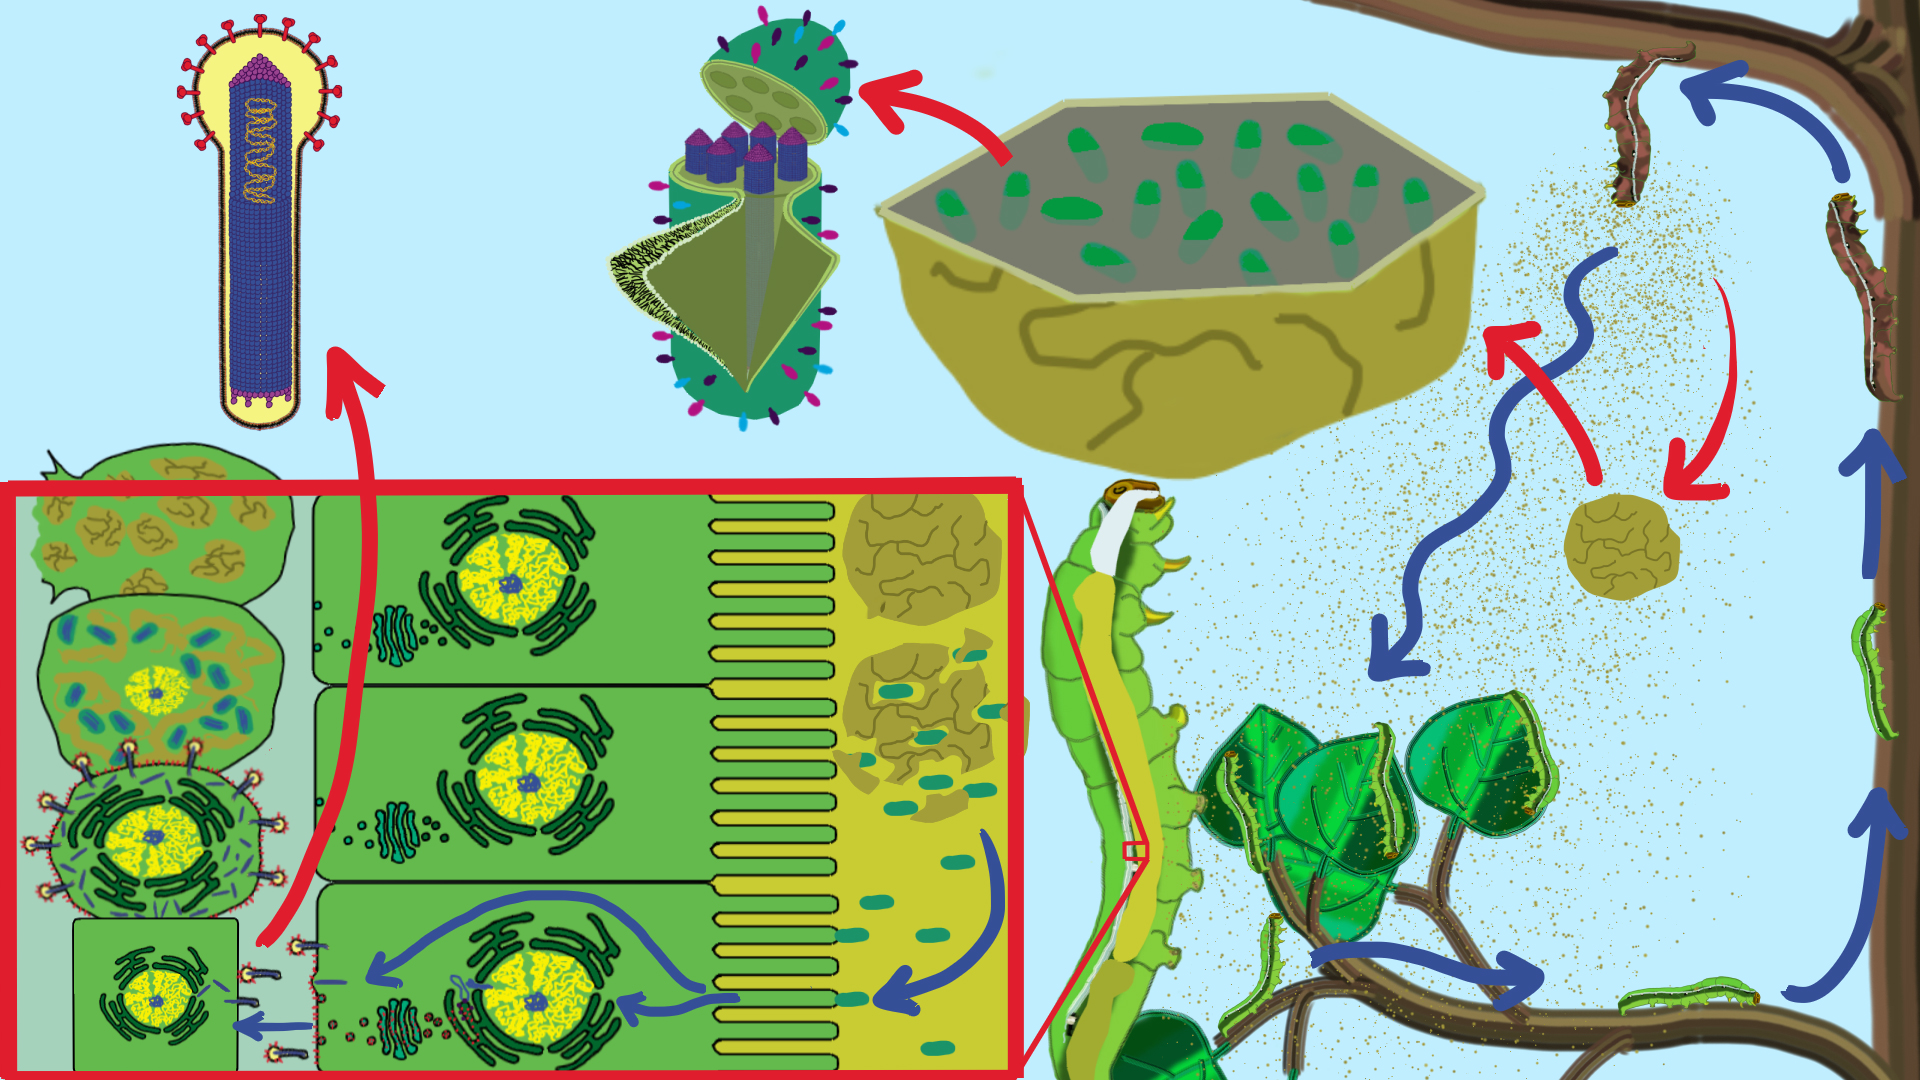
\includegraphics[width=0.8\linewidth]{figures/baculovirus_final} \caption{Ciclo de vida de los baculovirus y proceso de zombificación. Autor: Roberto Nájera.}\label{fig:zombificacion}
\end{figure}

De vuelta a la zombificación viral, los baculovirus inducen en sus hospedadores cambios directos tanto en el comportamiento alimentario como en la selección de esporulación. Una vez infectan a las orugas de la polilla y de las mariposas por ingesta, una vez la población del virus establece una infección viable, las orugas ingieren hojas incesantemente, lo que proporciona nutrientes para la replicación del virus. Una vez la cantidad de nutrientes garantiza una elevada producción de viriones, la siguiente acción de las orugas zombis es desplazarse verticalmente en las ramas de los árboles hasta encontrar un lugar alto en el que se inmovilizan. Finalmente las células infectadas secretan enzimas que disuelven al animal, haciendo llover trozos de tejido, junto a los cuerpos de oclusión, a manera de alimento a la espera de futuros hospedadores (\citet{williams2017covert}).

\includegraphics[width=0.8\textwidth,height=\textheight]{./figures/Death_March_The_Zombie_Caterpillars_es.mp4}.

Zombificación viral, tomado de \citet{youtube}.

Así los virus a diferencia de los humanos, no se disfrazan una vez al año de zombis, en realidad la zombificación parece ser su forma de vida primordial, ya sea a nivel de transformación de células u organismos multicelulares.

Para comentarios o preguntas puedes escribirnos tanto en la versión en \href{https://www.facebook.com/BioViral/posts/284936346967015}{Facebook} del presente post o la versión en \href{https://www.youtube.com/watch?v=Taqv4eFDtpo}{YouTube}.

\hypertarget{plantPand}{%
\section{Pandemias virales a escala mundial en plantas.}\label{plantPand}}

\textbf{El virus Hosta X y los lirios de plátano.}

El enigmático mundo de los virus de las plantas ejemplifica y contrasta con el énfasis de la investigación científica en virología humana. Quizá uno de los mejores casos que ilustra este contraste es la pandemia mundial aún en curso (desde 1990) del mosaico del Hosta, a causa del Virus Hosta X (VHX).

VHX es un virus desnudo (sin membrana) cuyo genoma es una hebra sencilla de RNA con polaridad positiva (ssRNA+, es leído directamente por el ribosoma). VHX pertenece a la familia Potexvirus, donde se hallan importantes virus que afectan la economía mundial como ``POTato virus X'' (virus del que deriva el nombre de la familia), los virus de esta familia se caracterizan por infectar de manera especie-específica a sus huéspedes, es decir, VHX infecta exclusivamente a las plantas del género Hosta, plantas con un alto valor en el mercado por su uso ornamental. Estas plantas son conocidas en Latinoamérica como lirios de plátano o simplemente Hosta. Son plantas muy comunes en diversos jardines del mundo, sin embargo suelen crecer principalmente en climas templados y estacionales, aunque aún así son apreciadas en jardinería a nivel mundial (\citet{baker2013hosta}).

\begin{figure}
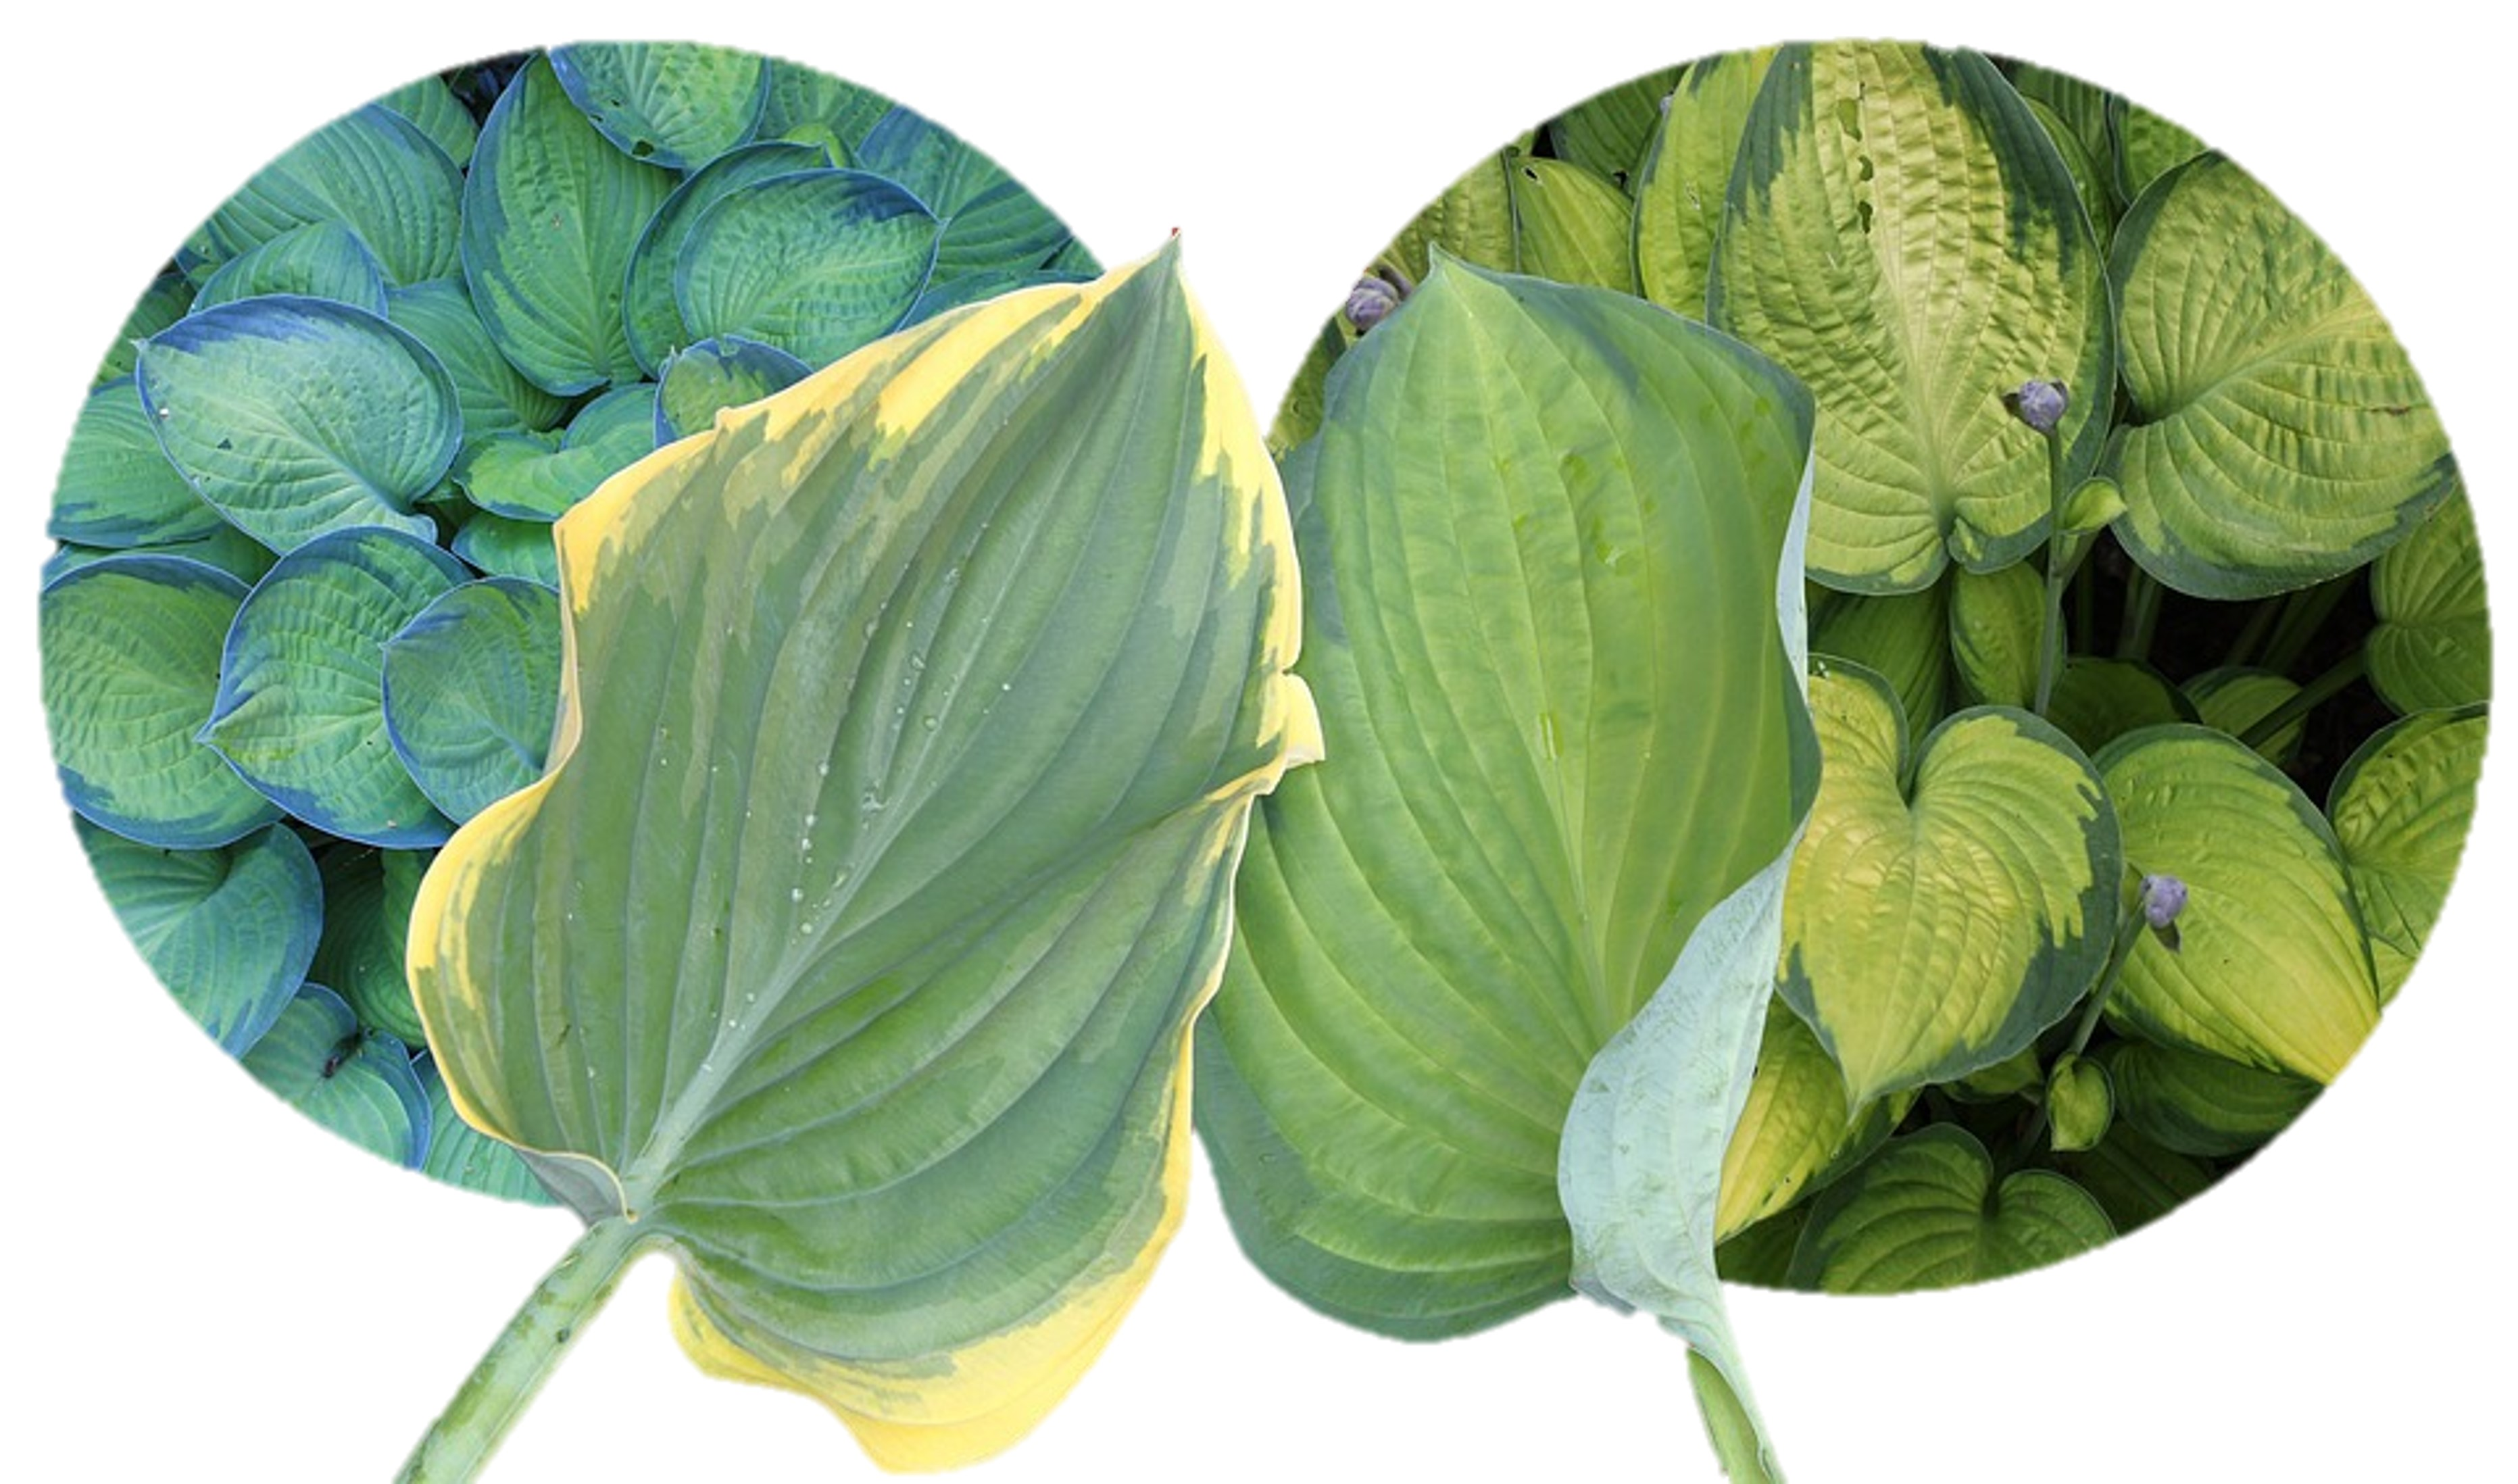
\includegraphics[width=0.6\linewidth]{figures/hosta_patterns} \caption{Ejemplares de lirio de plátano empleados en jardinería, exhibiendo patrones de pigmentación variegada por domesticación y no por infección viral}\label{fig:hosta}
\end{figure}

El estado de desconocimiento de la prevalencia del VHX, para antes del descubrimiento del virus, era tal que entre los coleccionistas expertos se describieron como cultivares o variedades de Hosta a las plantas ``Break Dance'', ``Eternal Father'', ``Leopard Frog'', ``Blue Freckles'' y ``Lunacy'', cuando en realidad son variedades clásicas cuyos patrones morfológicos diagnósticos no son producto de la diversificación de las variedades, sino más bien consecuencia de la infección del virus VHX (\citet{valverde2012viruses}).

La infección de VHX presenta como síntomas o consecuencias visibles mosaicos moteados verde-oscuro o amarillo-verdosos, además de distorsión de las hojas en forma de rugosidades. No obstante, dada la reproducibilidad parcial de dichas estructuras dichos cultivares despertaron bastante interés comercial, distribuyéndose entre especialistas y aficionados de todo el mundo.

La dificultad en el control de dicho virus radica en que los síntomas se manifiestan después de los 3 primeros años de cultivo en adelante, y aunque las plantas presentan una baja mortalidad, la elevada transmisibilidad de VHX al ser capaz de contagiarse, incluso por contacto con herramientas de jardinería o mediante transferencia entre raíces, ha dificultado frenar su propagación (\citet{valverde2012viruses}).

\begin{figure}
\includegraphics[width=0.4\linewidth]{figures/HVX_collage} \caption{Síntomas de la infección del virus Hosta X en cuatro variedades de lirios de plátano}\label{fig:hostaX}
\end{figure}

A diferencia de las epidemias en animales, dada la nula inmunidad que presentan las plantas domesticadas, la única forma de controlar la propagación del virus es la quema total de ejemplares con síntomas inequívocamente determinados. Dado a que el virus fluye por la savia de la planta, el estado de infección aún si es asintomática es sistémica.

Es importante resaltar que no todos los patrones de coloración o forma irregular en ejemplares de Hosta deriva de la infección viral, el criterio discriminante es la heredabilidad variable de dichos patrones, pues, el virus es capaz de transmitirse incluso por semillas, pero es incapaz de reproducir de manera idéntica o parecida el patrón en mosaico de las plantas descendientes.

\hypertarget{hiperendemia-del-virus-del-dengue.}{%
\section{Hiperendemia del virus del Dengue.}\label{hiperendemia-del-virus-del-dengue.}}

\textbf{50 años de circulación endémica en más de 100 países.}

El virus del Dengue y la situación epidemiológica que este causa es un gran modelo para comprender el significado de una enfermedad viral endémica, escenario al que llegaremos en el futuro cercano de la pandemia de COVID-19.

El dengue es una enfermedad viral transmitida por mosquitos (arboviral) principalmente de la especie \emph{Aedes aegypti} y, en menor grado, de la especie \emph{Ae. albopictus}. Es uno de los principales problemas sin vacunas eficaces de salud pública en las regiones tropicales y subtropicales. Por el carácter endémico de la enfermedad, esto es, por su circulación constante a lo largo del tiempo y de un modo predecible, cada año, alrededor de 400 millones de personas se infectan por el virus del dengue, con una tasa de mortalidad de alrededor del 20\% entre los pacientes con dengue grave sin tratamiento, frente a 1.5 a 2\% bajo cuidado médico (\citet{luang2018hyperendemic}). De allí que, una enfermedad viral endémica no es una enfermedad con repercusiones similares a la influenza.

Dado los efectos del cambio climático, las poblaciones del mosquito vector han logrado, en los últimos años, propagarse rápidamente a todas las regiones tropicales y subtropicales del mundo, además de países estacionales de las zonas limítrofes. Sin embargo, la enfermedad está muy extendida en los trópicos, con variaciones locales en el riesgo que dependen de parámetros climáticos, factores sociales y ambientales (\citet{luang2018hyperendemic}).

El virus del dengue (DENV) es un virus de ARN monocatenario de sentido positivo de la familia Flaviviridae. Su conformación genómica y organización como partícula viral o virión se muestra en la figura 1. El genoma, con tan solo 10.7Kb, posee dos regiones UTR en el extremo 5' y 3' respectivamente. Entre estas regiones existe un marco abierto de lectura (ORF) que codifica para 3 proteínas estructurales C (capside) , PrM (preMembrana) y E (envoltura) y para 7 proteínas no estructurales. Las regiones UTR y los bucles que se crean en ellas son de especial importancia en la asociación del material genético viral al ribosoma, mediando los cambios conformacionales en el genoma viral que facilitan su replicación (\citet{nanaware2021dengue}).

\begin{figure}
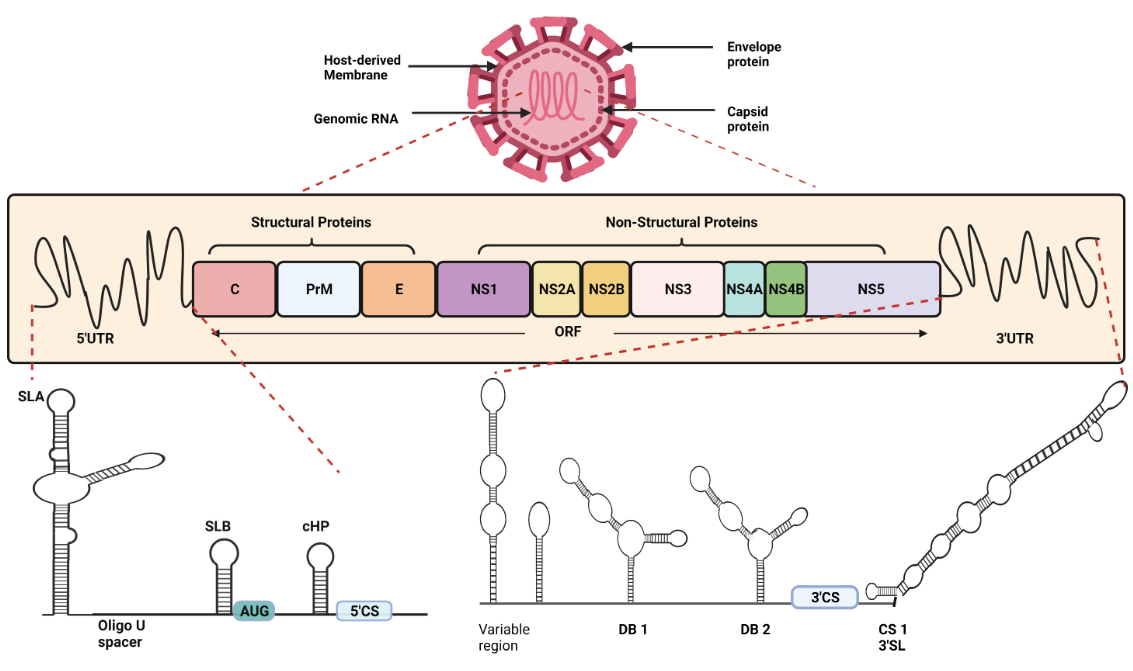
\includegraphics[width=0.8\linewidth]{figures/DenvFigura1} \caption{Conformación genómica y organización como partícula viral o virión. El virus del dengue (DENV) es un virus de ARN monocatenario de sentido positivo de la familia Flaviviridae. El genoma, con tan solo 10.7Kb,  posee dos regiones UTR en el extremo 5’ y 3’ respectivamente, tomado de @nanaware2021dengue}\label{fig:genomeDenv}
\end{figure}

Al igual que otros virus de ARN, el DENV presenta una considerable diversidad genética, presenta una tasa de mutación de 5.5 nucleótidos por año. A razón de esto, actualmente el virus se ha diversificado en cuatro linajes genéticos, que a su vez presentan 4 serotipos antigénicamente distintos (DENV-1-DENV-4), es decir que cada linaje genético se diferencia inmunológicamente mediante pruebas de neutralización de suero (\citet{nanaware2021dengue}). En la figura 2 se muestra un árbol filogenético de los 4 serotipos conocidos actualmente, junto a la diversidad de cambios de aminoácidos que se han registrado en distintas partes del \href{https://nextstrain.org/dengue/all}{genoma del virus y sus serotipos} (\citet{hadfield2018nextstrain}).\\
~\\

\begin{figure}
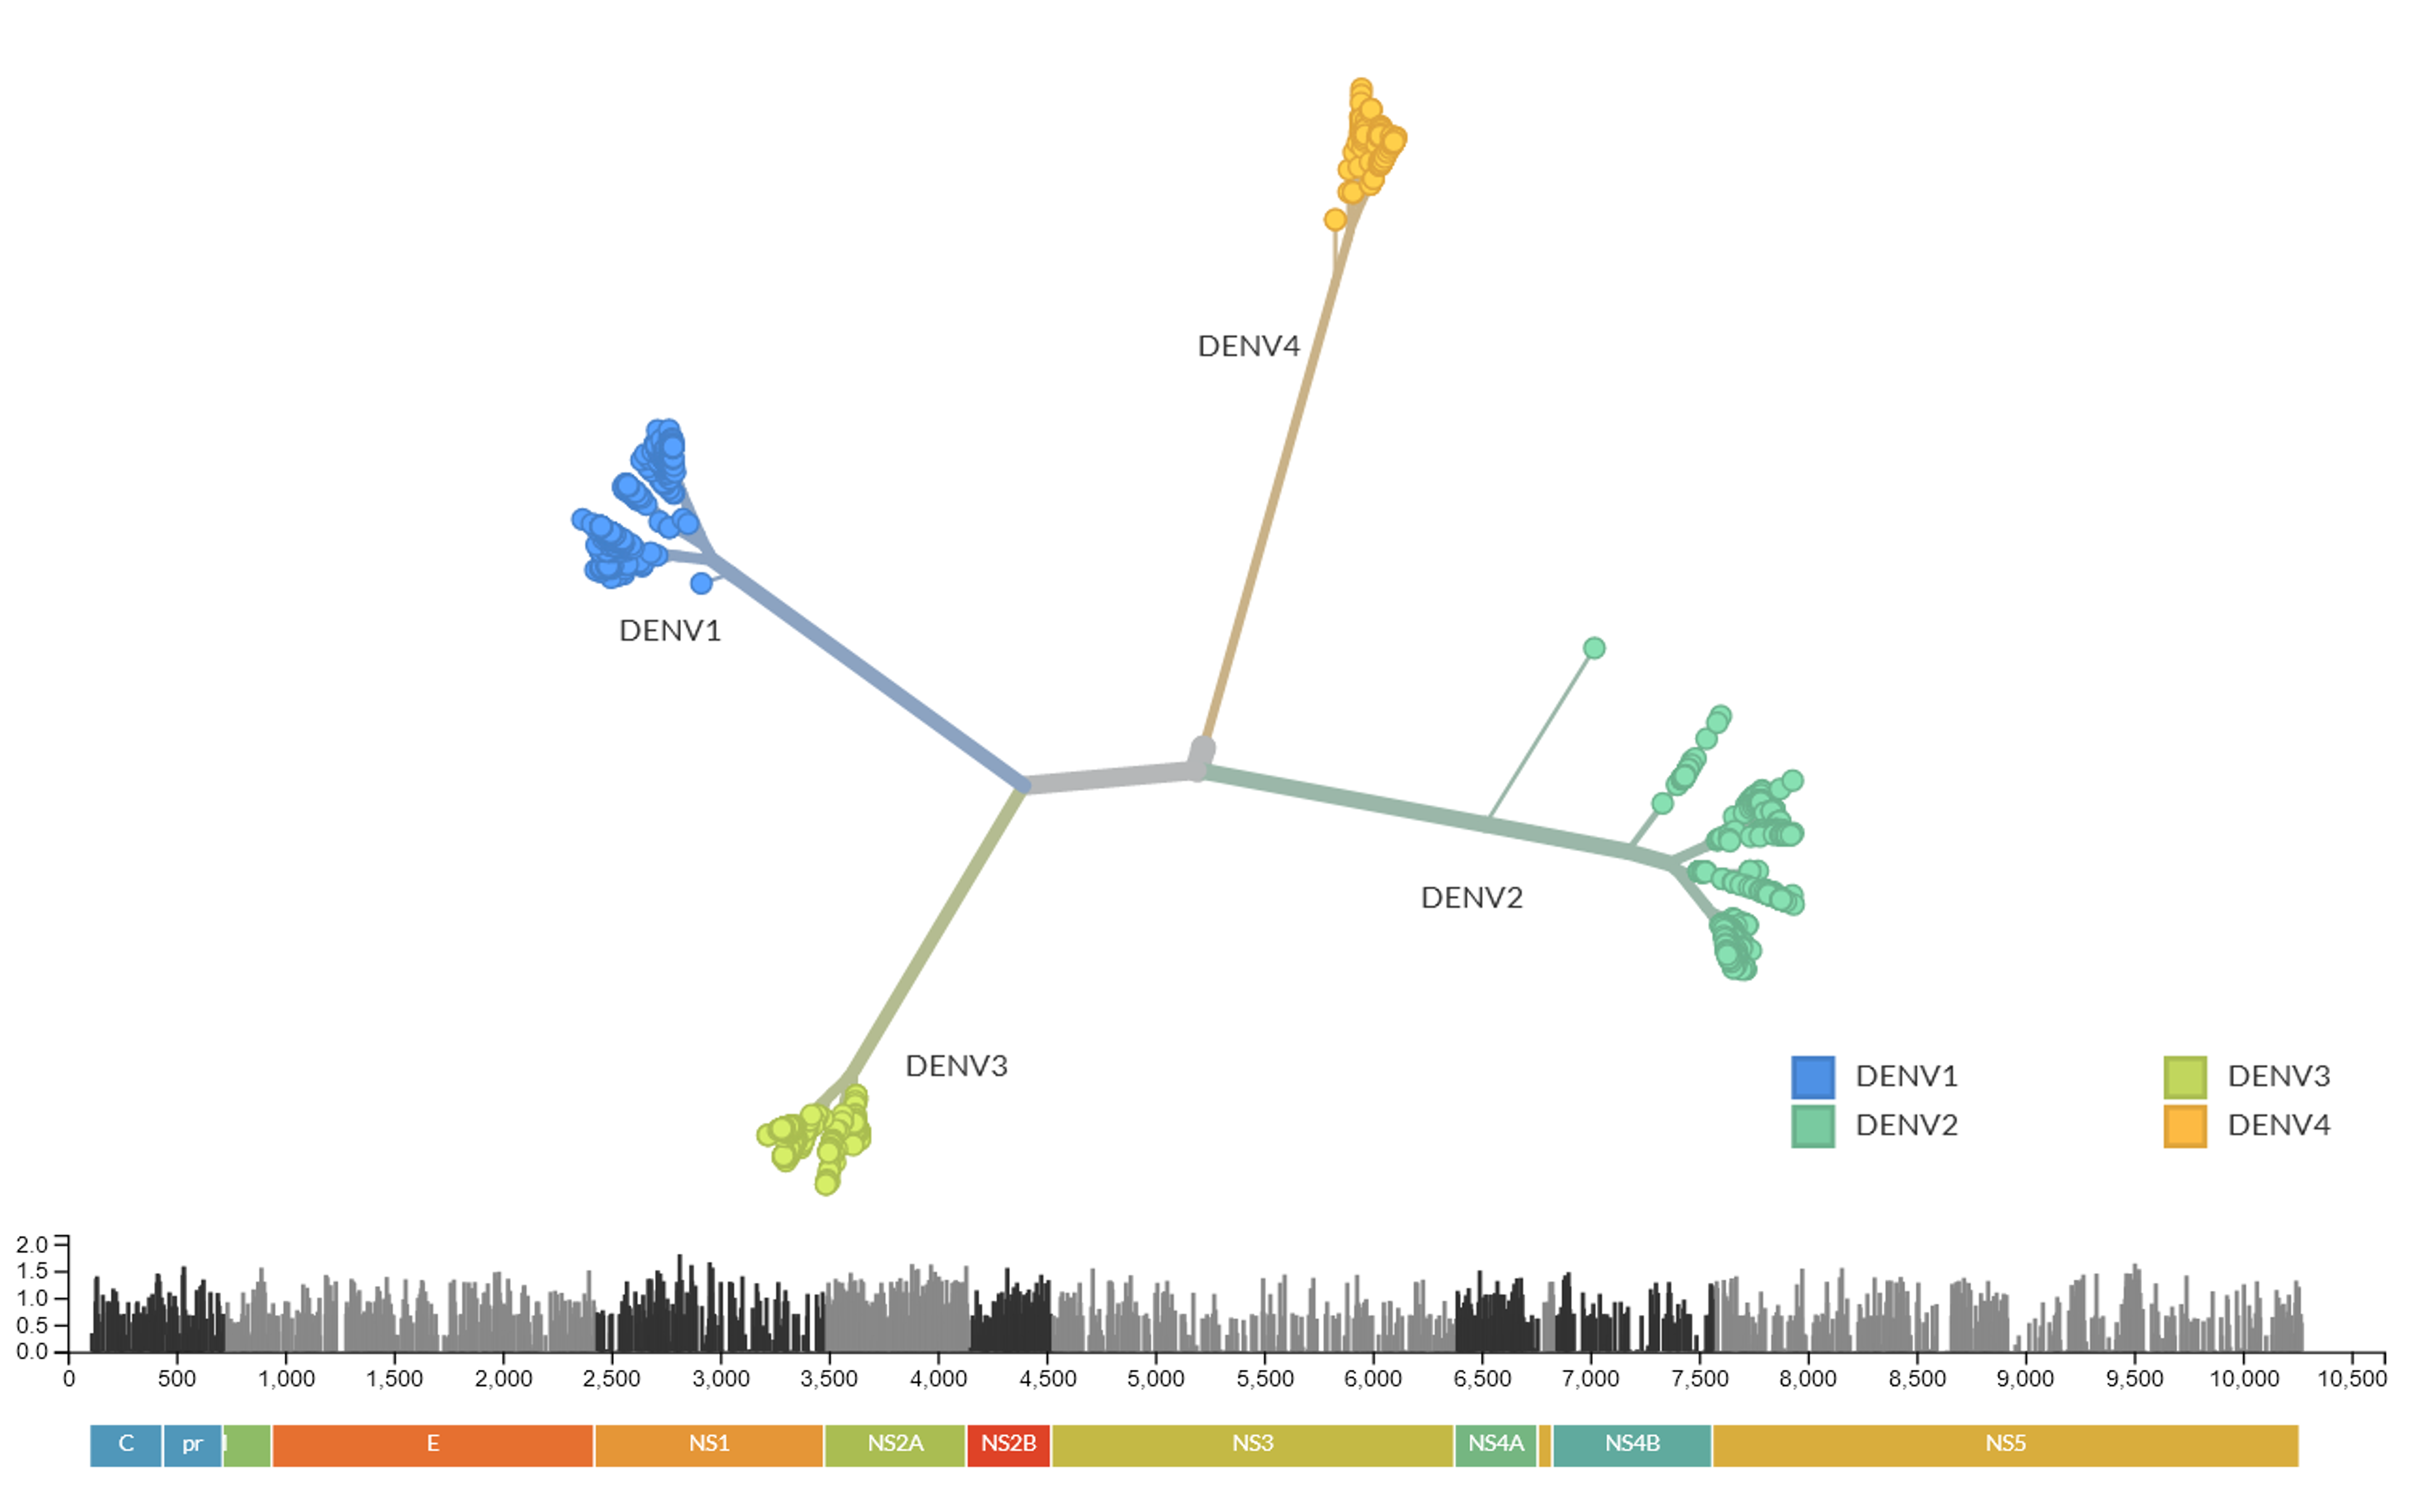
\includegraphics[width=0.8\linewidth]{figures/DenvFigura2} \caption{Árbol filogenético de los 4 serotipos conocidos actualmente, junto a la diversidad de cambios de aminoácidos que se han registrado en distintas partes del genoma del virus y sus serotipos, tomado de @hadfield2018nextstrain.}\label{fig:DenvSerotypes}
\end{figure}

Análisis filogenéticos de las secuencias de pacientes infectados con el virus permiten realizar comparaciones en la divergencia entre los serotipos existentes y ayudan a predecir posibles mutaciones que originan serotipos nuevos. En la figura 3 se muestra cómo a medida que pasa el tiempo se van acumulando cambios en cada uno de los distintos serotipos observándose una mayor acumulación de cambios en el serotipo DENV1 (\citet{hadfield2018nextstrain}).

\begin{figure}
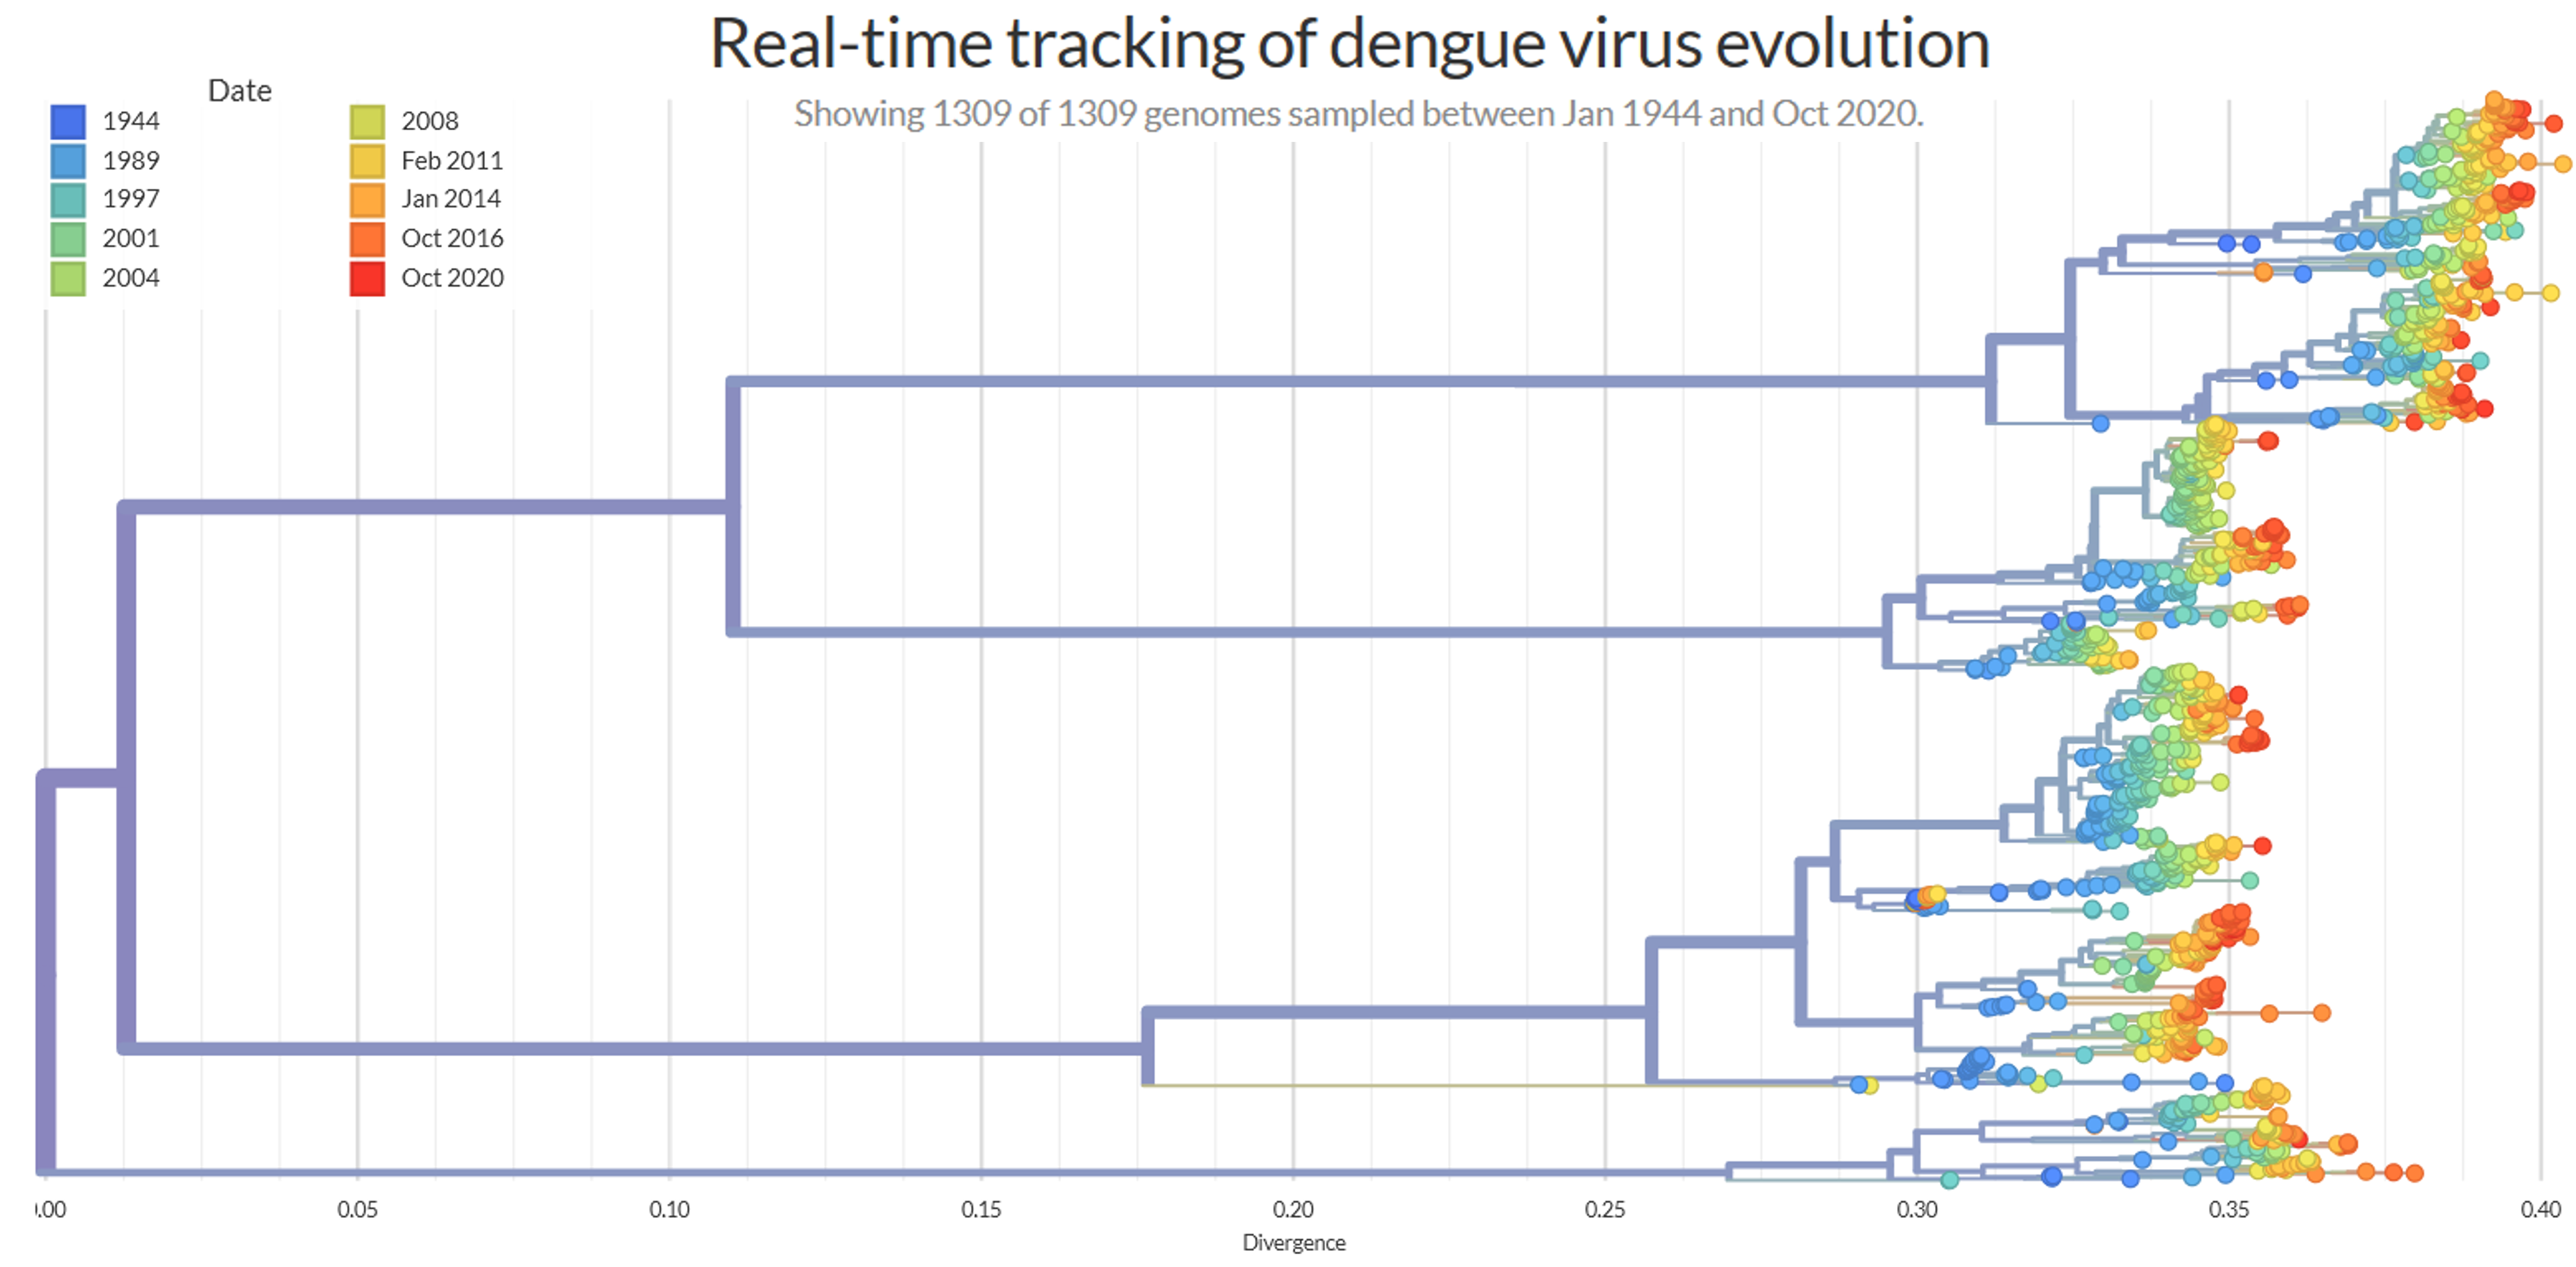
\includegraphics[width=0.8\linewidth]{figures/DenvFigura3} \caption{Filogenia en la que se ilustra el año de muestreo de cada secuencia empleada, se observa que, con el paso del tiempo se van acumulando cambios en cada uno de los distintos serotipos, sin embargo el serotipo DENV1 presenta la mayoría de cambios, lo que da lugar a una mayor divergencia., tomado de @hadfield2018nextstrain.}\label{fig:DenvPhyl}
\end{figure}

El ciclo de replicación viral se muestra en la figura 4. La partícula viral puede entrar a la célula humana huésped vía endocitosis, ya sea empleando receptores de la célula huésped o por endocitosis directa, mediada por anticuerpos, o mediada por recubrimiento con clatrina. Una vez dentro de la célula las partículas virales se translocan dentro de un endosoma al retículo endoplasmático donde se libera el RNA viral, el cual utiliza la maquinaria de replicación ribosómica para crear nuevas partículas virales inmaduras que son ensambladas en el complejo de Golgi, activadas mediante una maduración interpuesta por furina y finalmente liberadas vía exocitocis en la red trans de Golgi. Los cambios de pH dentro del endosoma y el exosoma son fundamentales para la replicación y la maduración del virus (\citet{nanaware2021dengue}).

\begin{figure}
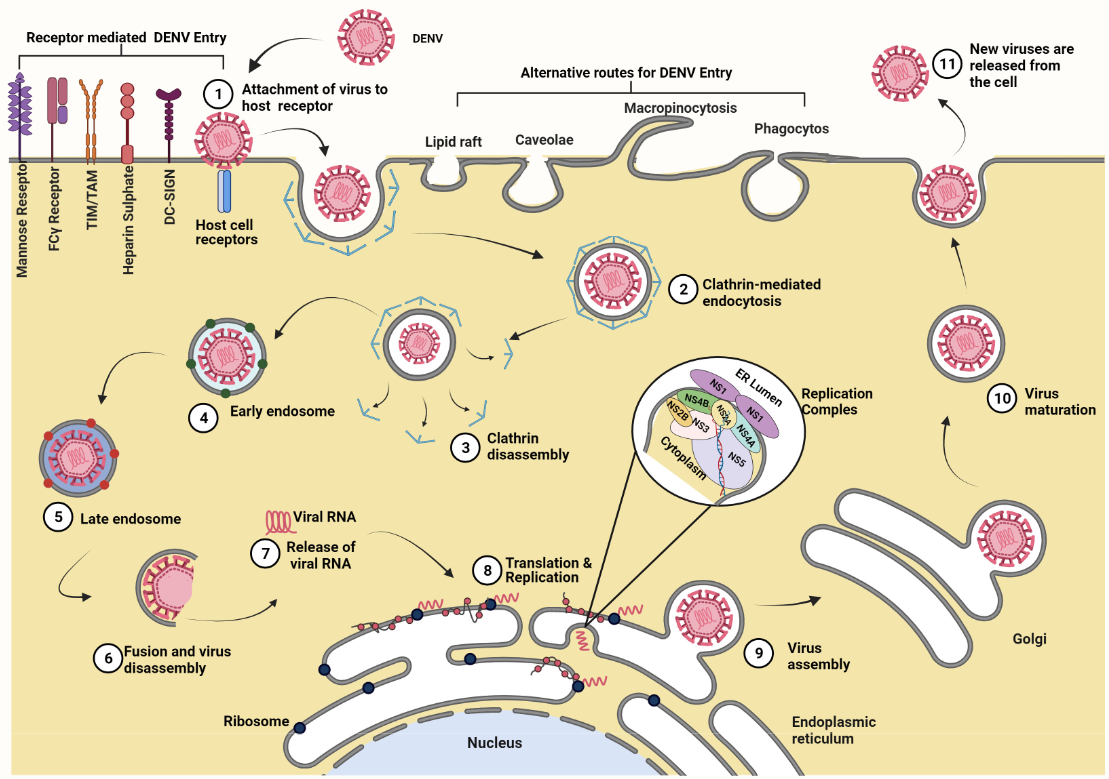
\includegraphics[width=0.8\linewidth]{figures/DenvFigura4} \caption{ La partícula viral puede entrar a la célula humana huésped vía endocitosis, ya sea empleando receptores de la célula huésped o por endocitosis directa, mediada por anticuerpos, o mediada por recubrimiento con clatrina. Una vez dentro de la célula las partículas virales se translocan dentro de un endosoma al retículo endoplasmático donde se libera el RNA viral, el cual utiliza la maquinaria de replicación ribosómica para crear nuevas partículas virales inmaduras que son ensambladas en el complejo de Golgi, activadas mediante una maduración interpuesta por furina y finalmente liberadas vía exocitocis en la red trans de Golgi. Los cambios de pH dentro del endosoma y el exosoma son fundamentales para la replicación y la maduración del virus, tomado de @nanaware2021dengue.}\label{fig:DenvCiclo}
\end{figure}

\hfill\break
Antes de 1970, solo nueve países habían sufrido epidemias de dengue grave. En la actualidad, la enfermedad es endémica en más de 100 países de las regiones de África, las Américas, el Mediterráneo Oriental, Asia Sudoriental y el Pacífico Occidental. Las regiones más gravemente afectadas son las Américas, Asia Sudoriental y el Pacífico Occidental; en Asia se concentra aproximadamente el 70\% de la carga mundial de la enfermedad (\citet{whodenv}). Además del aumento del número de casos debido a la propagación de la enfermedad a nuevas zonas, entre ellas Europa, también se producen brotes epidémicos de carácter explosivo (\citet{hadfield2018nextstrain}).

Se piensa que luego de la primera y la segunda guerra mundial, se empezó a diseminar el virus y el mosquito vector a numerosas partes del mundo desde el sudeste asiático. Esto ha provocado la condición hiperendémica actual de la enfermedad (\citet{hadfield2018nextstrain}). Situación que acontece cuando circulan los 4 distintos serotipos en una misma región del planeta, como se ilustra en la figura 5. Nótese como en casi todas las regiones existen los 4 serotipos simultáneamente, y que estas frecuencias pueden y varían en el tiempo. Europa es la única región donde solo hay dos serotipos DENV1 y DENV2. Y en las regiones nórdicas (donde el vector mosquito no habita) no existe el virus.

\begin{figure}
\includegraphics[width=0.8\linewidth]{figures/DenvFigura5} \caption{Hiperendemia mundial del virus Dengue. Distribución de los 4 serotipos por regiones. Aquellas regiones con presencia y circulación endógena de 4 serotipos se les denomina hiperendemia., tomado de @hadfield2018nextstrain}\label{fig:DenvHyper}
\end{figure}

\hypertarget{paleovir}{%
\section{Aplicaciones de la Paleo-Virología.}\label{paleovir}}

\textbf{La historia co-evolutiva entre retrovirus endógenos y su huésped humano refleja el patrón de migración de nuestra especie.}

Los humanos somos seres a los que nos gusta clasificar. Y nos gusta mucho más clasificarnos a nosotros mismos; así pues, tenemos nombres, apellidos, familias, tribus, nacionalidades, etc. Este afán por clasificar también está unido a una necesidad de conocer de dónde venimos, de cuál fue el recorrido de nuestros ancestros para llegar a donde estamos hoy en día (\citet{terrell1977biology}). Tradicionalmente estos estudios se hacen siguiendo registros de fósiles humanos, análisis arqueológicos, históricos, antropomórficos, socio-culturales y biogeográficos (\citet{terrell1977biology}).

Sin embargo, con el advenimiento de la era genómica esto ha cambiado radicalmente (\citet{kolb2013using}, \citet{wohns2022unified}, \citet{kajan2020virus}). Nuestra capacidad para determinar las relaciones entre individuos, poblaciones y especies se está transformando gracias a las colecciones en crecimiento, actualmente con miles de genomas obtenidos a partir de ADN antiguo, bases de datos de muestras de interés médico, a escala poblacional, sumado a los esfuerzos para secuenciar millones de especies eucariotas. Estas relaciones, y las distribuciones de la variación genética y fenotípica resultante, reflejan el complejo conjunto de procesos y acontecimientos selectivos, demográficos y moleculares que han dado forma a las especies y, por consiguiente, son una rica fuente de información sobre ellas (\citet{kolb2013using}, \citet{wohns2022unified}).

Recientemente, los métodos para lograr inferir estas relaciones poblacionales en el humano han presentado numerosos retos debido al volumen de información disponible y el reto que implica depurarla (\citet{wohns2022unified}). Estos estudios de genómica comparativa tienen el problema de poder llegar a ser costosos por muestra analizada, lo que restringe el número de muestras a utilizar, lo que conlleva a problemas de representación de las diversas etnias de la especie, y además, pueden dar resultados distintos, dependiendo de las regiones del genoma que se comparen o el método de estudio utilizados (SNLP, RFLP, ARN16s, etc.) (\citet{kolb2013using}, \citet{wohns2022unified}). Pero en particular, la variabilidad genética de estos marcadores limita la resolución temporal a evaluar, en otras palabras, la tasa de mutación en estas secuencias humanas es mucho más lenta que la tasa de migración.

Debido a lo anterior expuesto, nuevos y mejores métodos para indagar sobre nuestra biogeografía se encuentran en desarrollo. Uno de los métodos novedosos propuestos es la utilización de secuencias del viroma humano, es decir retro-virus endógenos activos, cuya mutación, al ser mucho mayor que las secuencias no-virales del genoma humano, permiten indagar escalas temporales cercanas a las empleadas en el estudio de las migraciones humanas (\citet{kolb2013using}).

Los virus representan buenos candidatos para estos estudios debido a la íntima co-evolución que se da entre el virus y el huésped, donde una carrera de competencia (arms race) entre factores virulentos del virus y la respuesta del huésped moldean eventos de introducción, expulsión del genoma, eventos evolutivos que nos permiten calibrar relojes moleculares y otros aspectos de la biología de ambos organismos, principalmente a través del análisis de eventos de recombinación (\citet{kolb2013using}).

\textbackslash begin\{figure\}
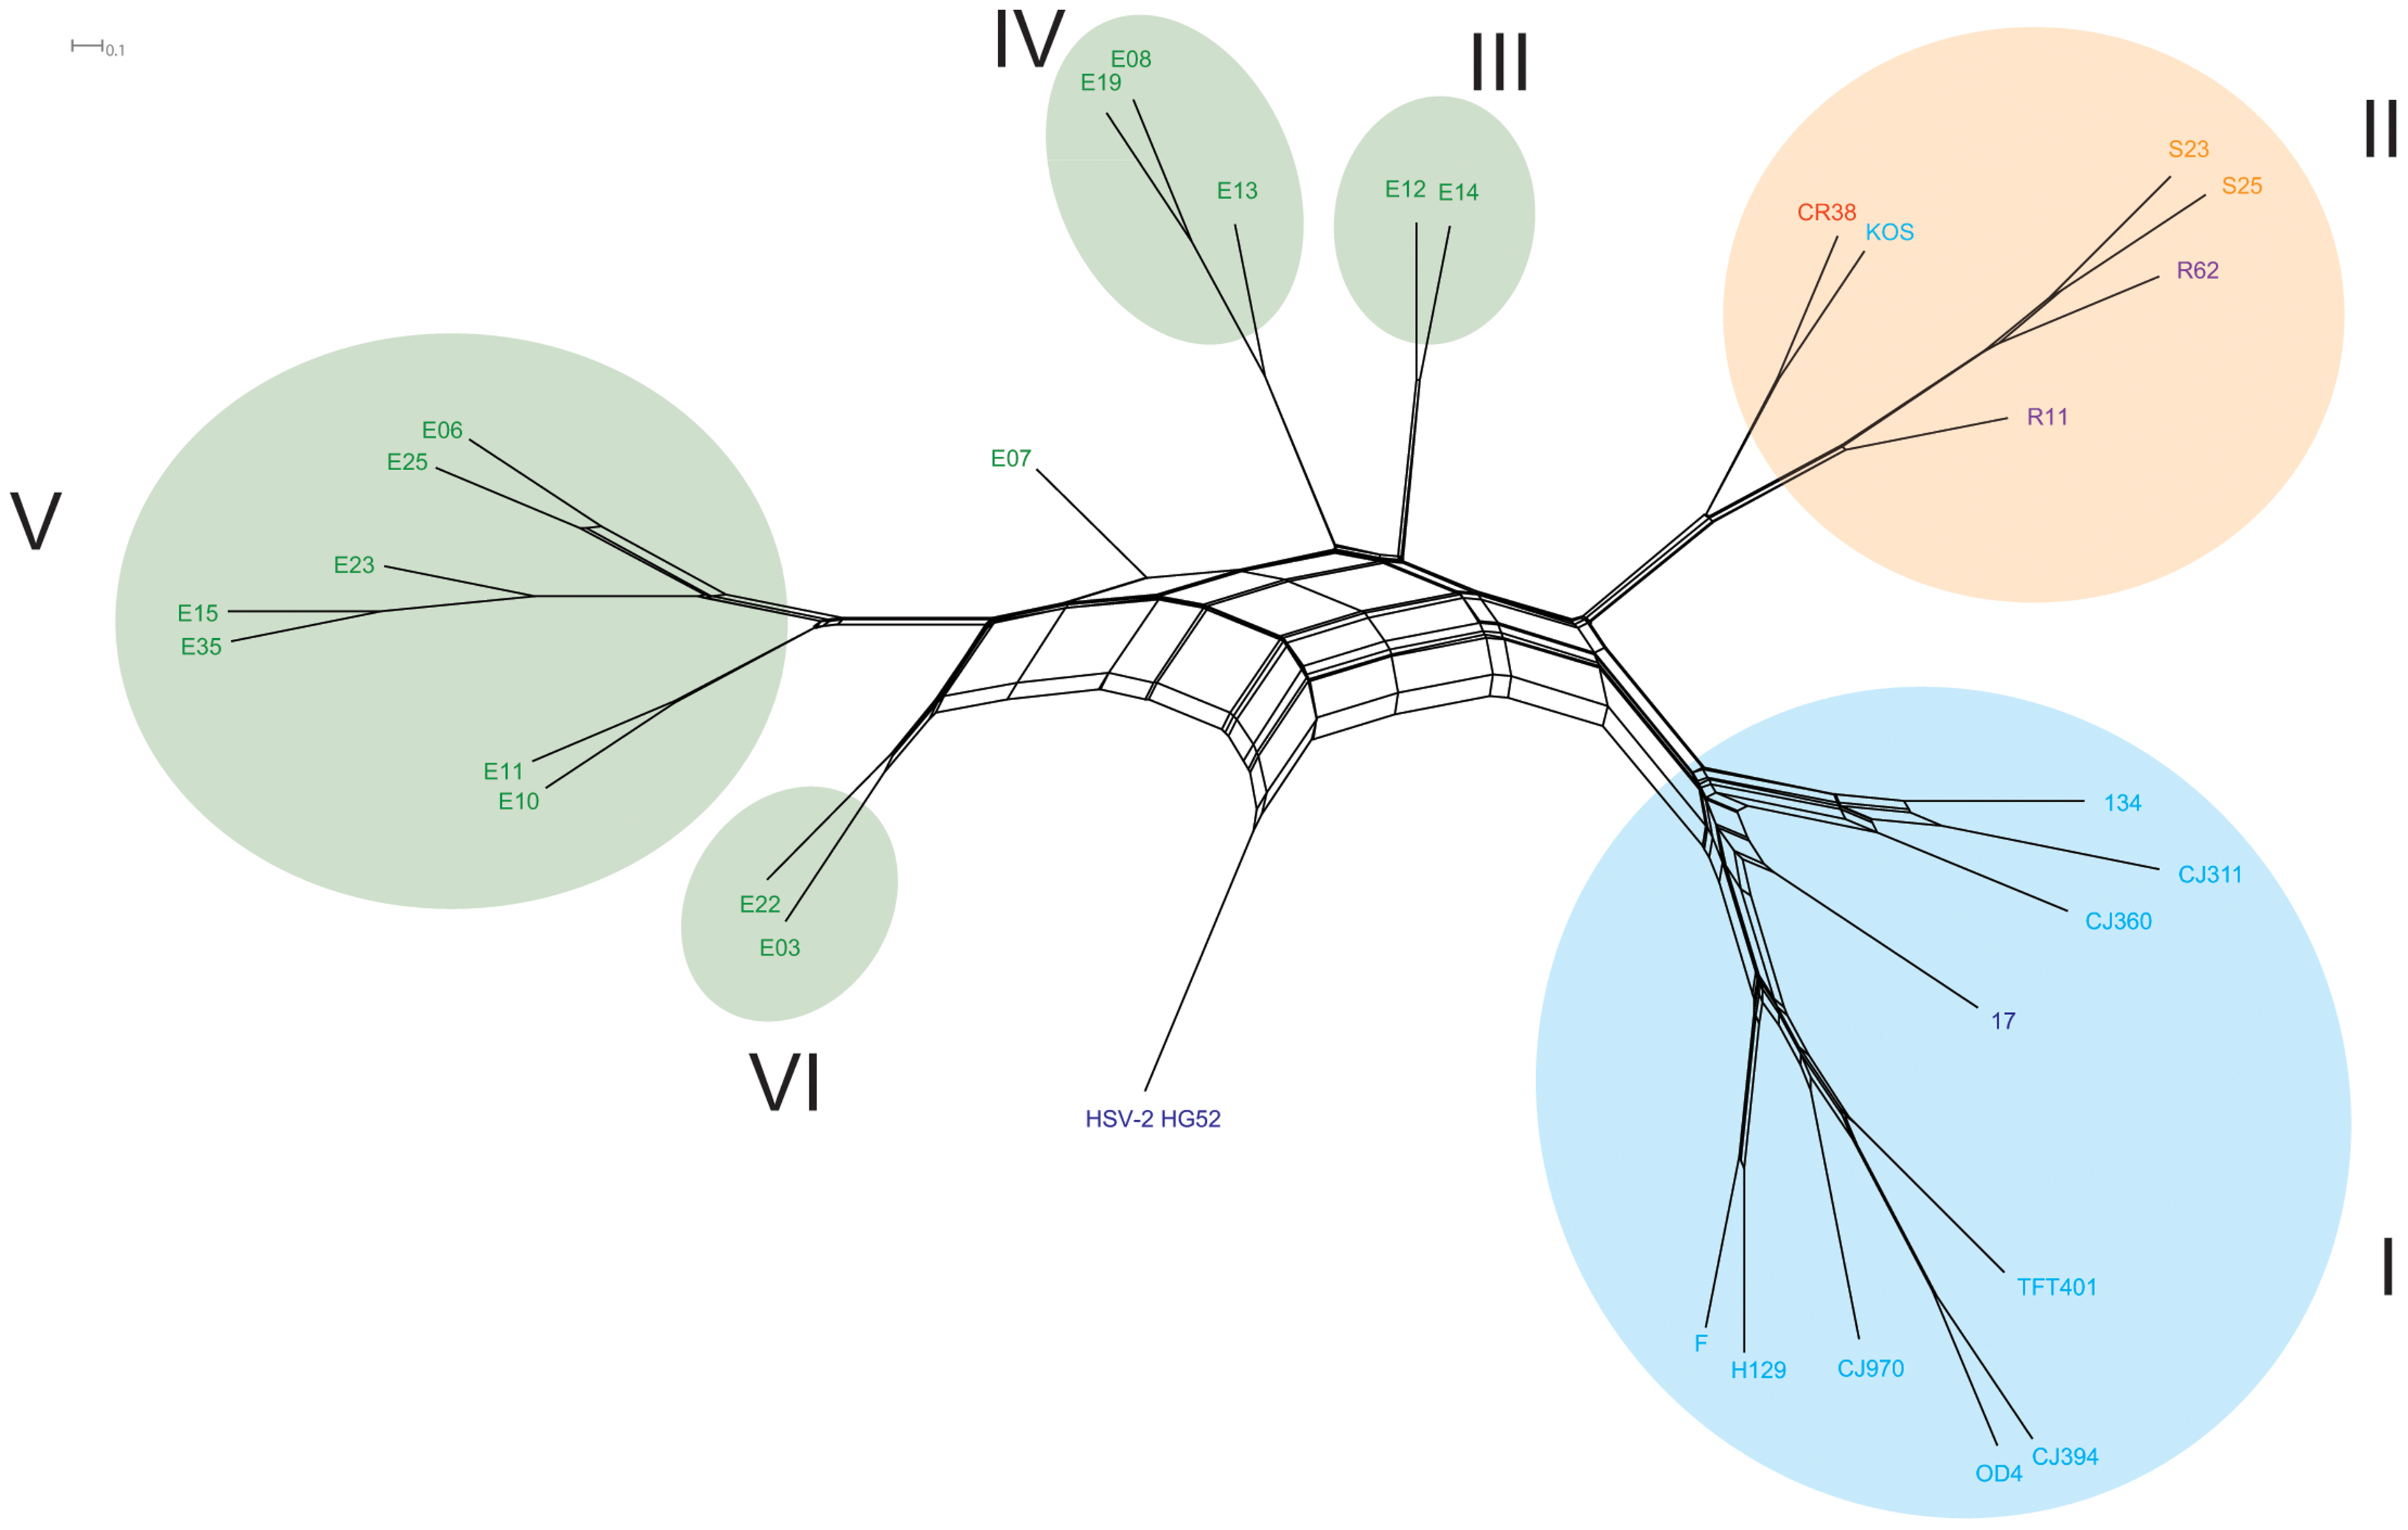
\includegraphics[width=0.8\linewidth]{figures/VHS1} \textbackslash caption\{Árbol de secuencias consenso construido de una partición de 5kb del genoma del virus examinado mediante un análisis boostrap de máxima similitud con 500 repeticiones. Un consenso del 70\% se usó como valor umbral para realizar las agrupaciones. El clado I corresponde a poblaciones norteamericanas y europeas , el clado II americanas y del asía oriental y los clados IIIV V y VI son de áfrica del éste. HSPV-2 se utilizó como grupo comparativo de afuera, tomado de \citet{kolb2013using}\}\label{fig:sixclades}
\textbackslash end\{figure\}

Los virus humanos siendo organismos de fácil secuenciamiento, en términos de la diminuta escala del genoma, y por lo general altamente conservados, este hecho ha permitido el desarrollo de una nueva especialidad en la virología evolutiva denominada paleo-virología, la cual, a partir del estudio de la coevolución huésped-parásito, se aproxima al entendimiento de eventos históricos de las especies, como la migración de las poblaciones humanas desde el lugar de origen, hasta el alcance de la distribución mundial.

El virus del herpes simple (VHS-1) es un candidato que ha mostrado ser ideal para este tipo de análisis. Los herpesvirus son grandes virus de ADN de doble cadena con genomas que varían en tamaño de 124 a 295 kilobases. La subfamilia de los alfaherpesvirus se caracteriza por la capacidad de establecer infecciones latentes en los ganglios nerviosos sensoriales. Estudios filogenéticos anteriores han demostrado que los herpesvirus han coevolucionado con sus huéspedes. El virus del herpes simple tipo 1 (HSV-1) es un alfaherpesvirus con un genoma de aproximadamente 152 Kb. El VHS-1 causa lesiones mucocutáneas orales, así como queratitis y encefalitis, y es un importante patógeno humano (\citet{kolb2013using})

Mediante análisis filogenéticos y frecuencias de recombinación se ha determinado que el VHS-1 presenta una estructura mínima de seis clados, cada uno correlacionado con regiones geográficas distintas. Los datos filogenéticos de las tasas de sustitución del VHS-1 sugiere una tasa de aproximadamente 1,38*10\^{}7 subs/sitio/año. El análisis de recombinación del VHS-1 muestra evidencias de recombinación inter e intracladística (es decir recombinación dentro del mismo linaje) (\citet{kolb2013using}).

Estas características del virus se han utilizado en un muestreo global de cepas de VHS-1 para el análisis filogenético y apoya la conclusión de que las cepas de VHS-1 han co-migrado con sus huéspedes humanos, dando lugar a clados virales geográficamente separados (\citet{kolb2013using}). En la figura 2 se puede observar como la historia evolutiva de cada clado de VHS-1 correlaciona geográfica y temporalmente, con los eventos migratorios y de separación geográfica de los grandes grupos de poblaciones humanas existentes a lo largo del tiempo (\citet{kolb2013using}).

\begin{figure}
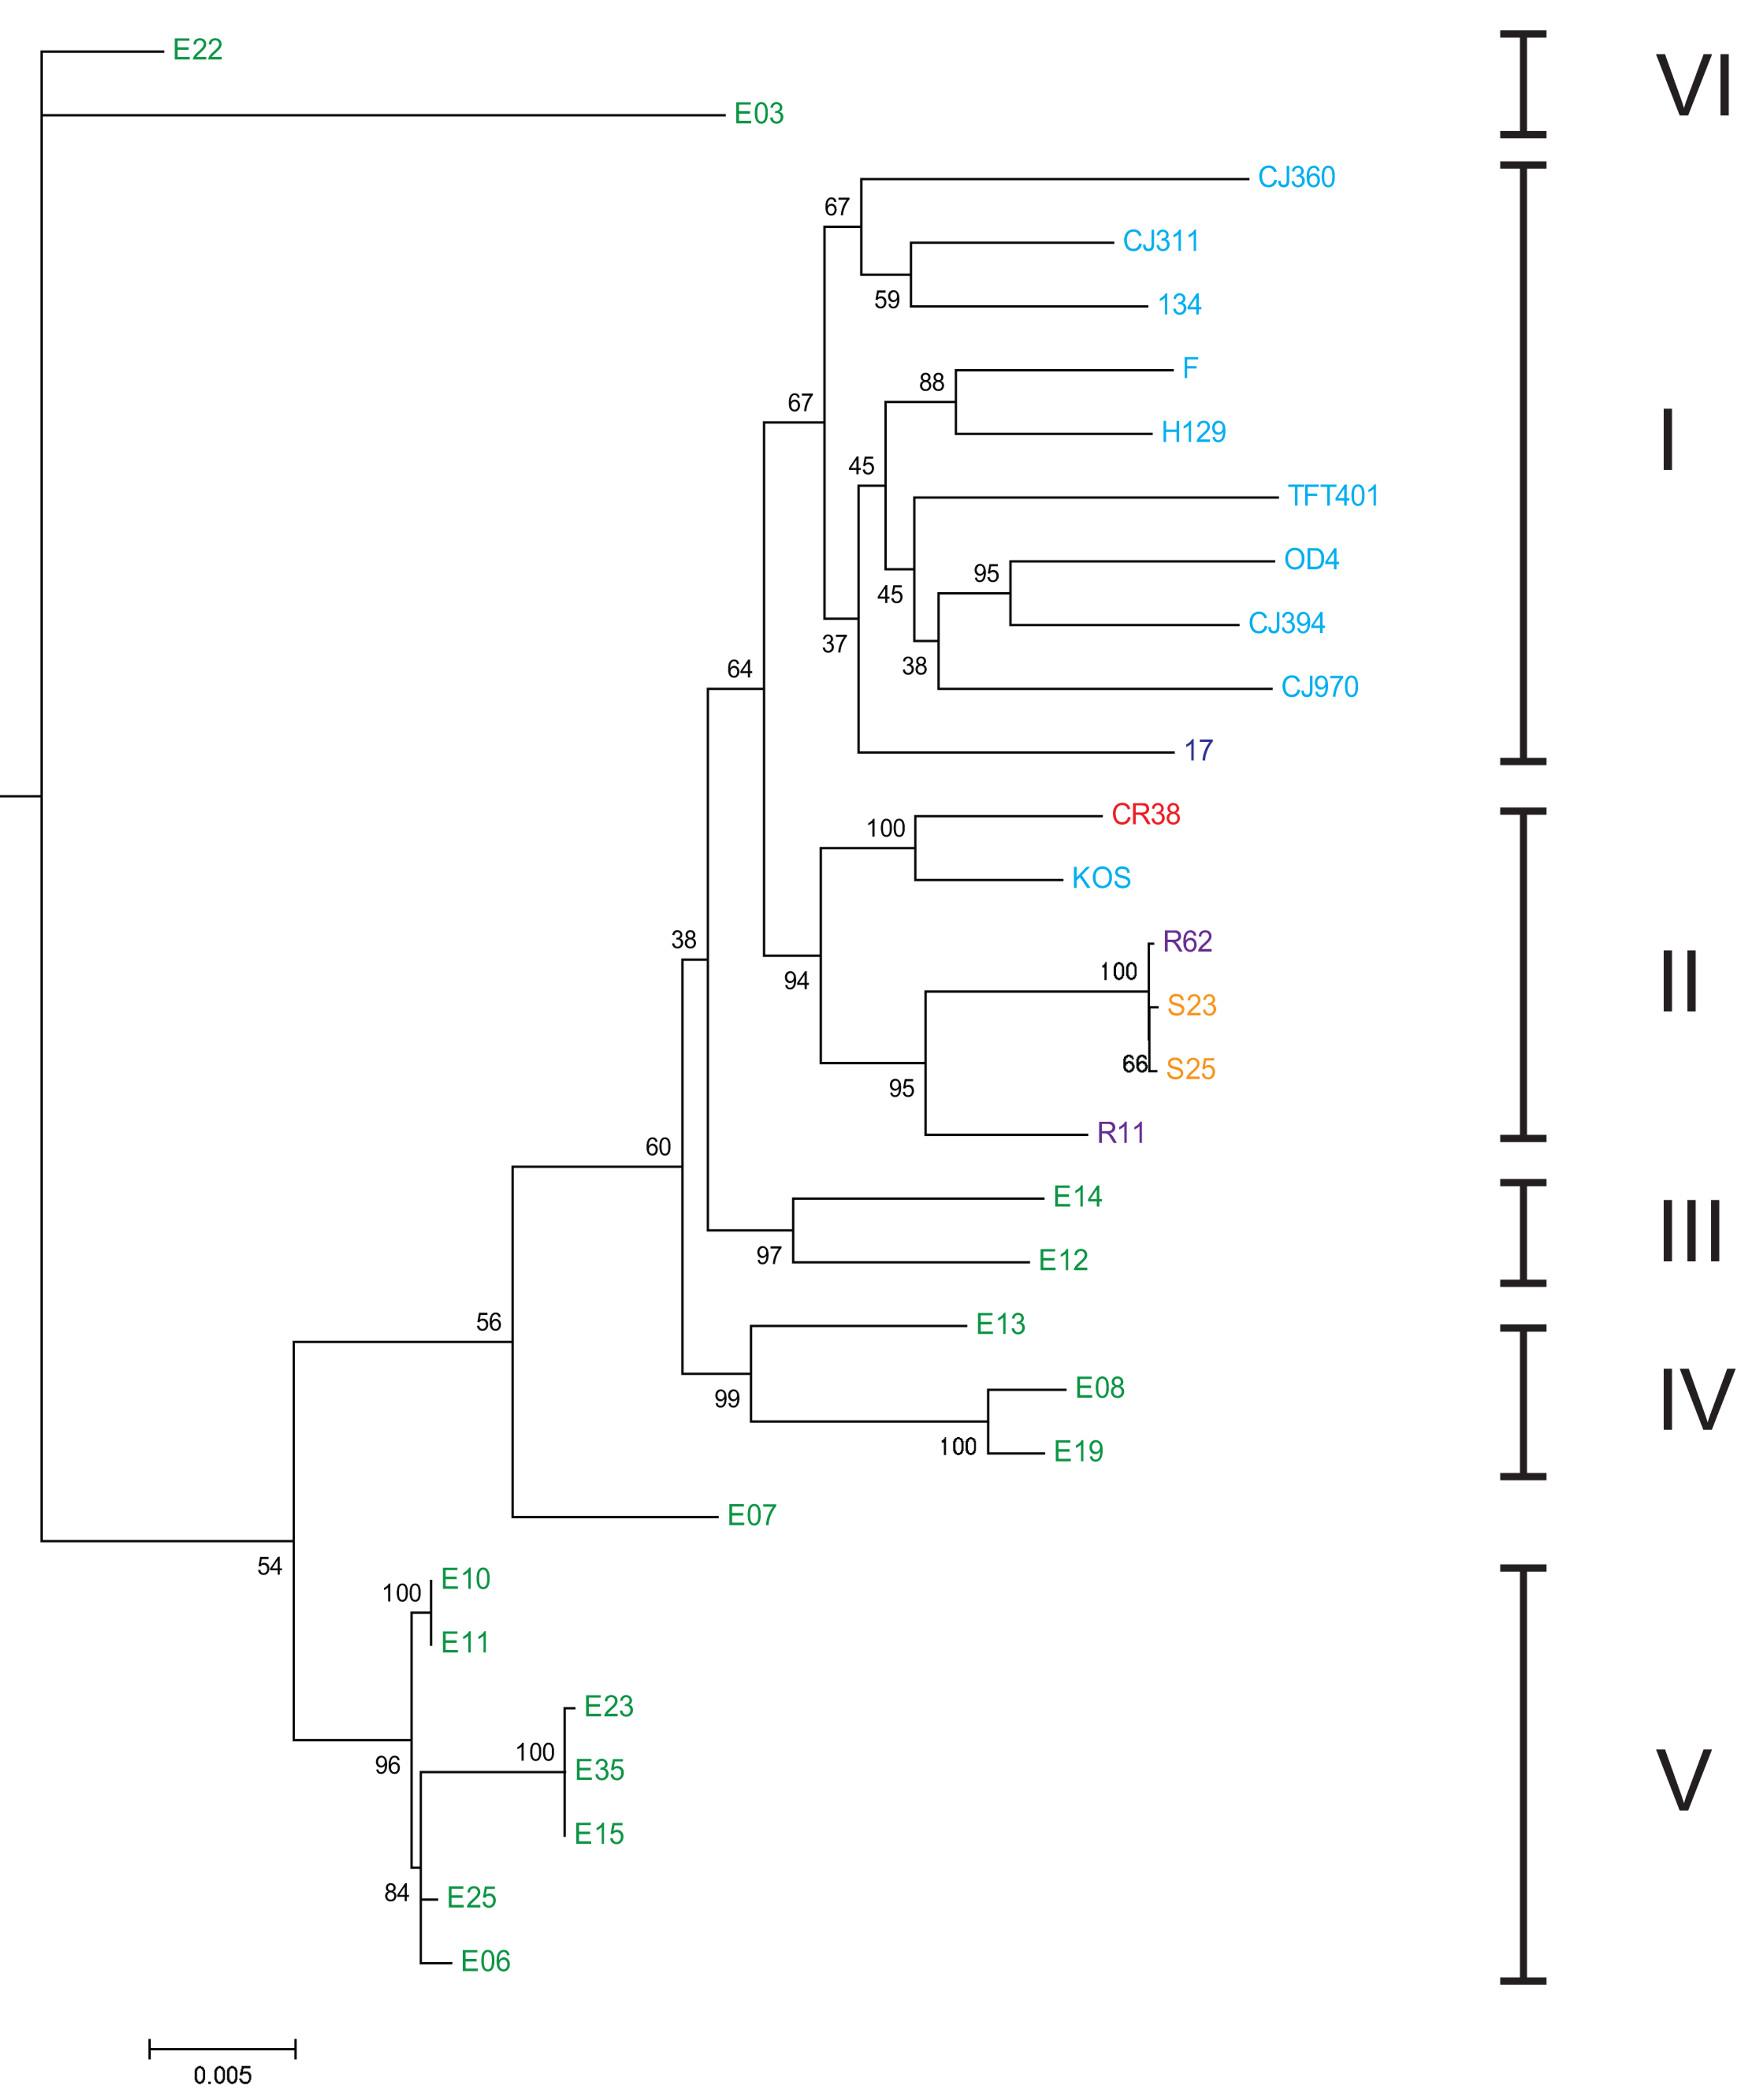
\includegraphics[width=0.8\linewidth]{figures/VHS2} \caption{Árbol filogenético ML enraizado (HSV-2 se uso como grupo externo) de las distintas variedades de VHS-1 y su correlación con los 6 grupos de poblaciones humanas establecidas en en estudio (números latinos a la derecha). Nótese como cada clado corresponde a una población en particular, evidenciando una co-evolución del virus con cada población humana. De allí que el análisis de diversidad genética de HSV-2 resulta en  una herramienta de análisis de migración y biogeografía humana. Los aislados virales de poblaciones actuales están coloreados según el país de origen: EE.UU.: azul claro, Reino Unido: azul oscuro, China: rojo, Corea del Sur: púrpura, Japón: amarillo y Kenia: verde, tomado de @kolb2013using}\label{fig:sixcladesroot}
\end{figure}

La secuenciación múltiple de los genomas del VHS-1 reduce significativamente el costo de secuenciamiento a escala genómica humana, por lo que los marcadores paleovirales se establecen como grandes sustitutos, no solo por ventaja económica, sino que también a nivel de la complejidad de los análisis computacionales requeridos para el estudio de la migración humana.

A propósito, el reciente estudio de la genealogía genómica humana, que se posiciona como el esfuerzo más exhaustivo hasta el momento, al emplear un total de 3,601 genomas humanos actuales y 8 genomas antiguos. La historia de las migraciones humanas inferida a partir del análisis del marcador viral VHS-1, no dista significativamente de la propuesta genealógica reciente, la cual es computacionalmente mucho más demandante.

\begin{figure}
\includegraphics[width=0.8\linewidth]{figures/VHS3} \caption{Comparación de las rutas migratorias del virus y los resultados del análsis genalógico de cerca de ~3600 genomas contemporaneos. Ambas aproximaciones dan soporte a la hipótesis del origen único del humano en el este del continente africano. Sin embargo, los eventos migratorios son capturados por la aproximación paleovirológica y no genealógica. Eventos de migración por tierra se representan con líneas amarillas; por aire/mar con la línea púrpura. Los países de origen de las cepas del presente estudio son China (rojo), Japón (naranja), Kenia (verde oscuro), Corea del Sur (púrpura), Reino Unido (azul oscuro) y Estados Unidos (azul claro). Tomado de @kolb2013using y @wohns2022unified}\label{fig:migratory}
\end{figure}

A manera de comparación, adjuntamos el video suplementario de la más reciente genealogía humana (\citet{kolb2013using} y @\citet{wohns2022unified}). Nótese que en ambos estudios se evidencia como origen único de todas las poblaciones humanas el este de áfrica, según el análisis de genomas humanos, hace unos 2 millones de años aproximadamente (80 mil generaciones). Mientras qué, este mismo hecho se evidencia en el tiempo estimado de divergencia de HSV-1 de HSV-2 es de 2.18 (±0.753) millones de años.

\includegraphics[width=0.8\textwidth,height=\textheight]{./figures/HumanMig.mp4}.

Localización estimada de los ancestros genéticos humanos: Una genealogía unificada de los genomas modernos y antiguos, tomado de \citet{wohns2022unified}

Con respecto a las diferencias entre ambos mapas, el sesgo muestral de los dos análisis prepondera la migración hacia américa vía Europa-Groenlandia, más no desde Asia, vía estrecho de Bering. No obstante, el agrupamiento de la cepa KOS (derivada de américa) con el clado asiático CR38 (derivado de China), R62 (Sur Corea), S23 y S25 (Japón), a diferencia del estudio genómico, aporta la resolución necesaria para no descartar que ambos escenarios migratorios ocurrieron.

En la tabla 1. se muestra cómo distintos eventos de la evolución y migración humana corresponden con distintos eventos de diversificación del virus HSV-2. Lo que permite ilustrar la resolución de esta herramienta y su capacidad para indagar sobre la historia evolutiva y migratoria del humano, como también de otras especies, ya que, toda vida celular es a su vez un consorcio de holobiontes, en el que habitan y co-evolucionan cientos de linajes de vida viral o virucelular.

\begin{longtable}[]{@{}
  >{\raggedright\arraybackslash}p{(\columnwidth - 4\tabcolsep) * \real{0.36}}
  >{\raggedleft\arraybackslash}p{(\columnwidth - 4\tabcolsep) * \real{0.22}}
  >{\raggedright\arraybackslash}p{(\columnwidth - 4\tabcolsep) * \real{0.41}}@{}}
\toprule
Divergencia entre cepa o especie de Virus & TMRCA & Evento en las poblaciones humanas \\
\midrule
\endhead
HSV-1 y HSV-2 & 2.184 ± 0.753 mya & Origen aproximado del H. sapines \\
Cepas de HSV-1 & 50.3 ± 16.7 kya & Emigración de África 60 kya \\
Cepas de Eurasia & 32.8 ± 10.9 kya & Migración Asia-Europa 20-40 kya \\
KOS y CR38 & 15.76 ± 5.3 kya & Poblamiento de América 12-20 kya \\
\bottomrule
\end{longtable}

Tabla 1. Divergencia viral estimada vs evidencia temporal de los registros arqueológicos de los eventos de migración humana, tomado y traducido de \citet{kolb2013using} TMRCA: Tiempo hasta el ancestro común más reciente.

El \href{https://www.youtube.com/watch?v=xqy2-m080jY}{video de la fuente} (\citet{wohns2022unified}) ha sido editado con la canción Val d'inverno del grupo italiano Evoca.

\backmatter

  \bibliography{book.bib,packages.bib,References\_Bibtex.bib}

\end{document}
